\documentclass[../Main.tex]{subfiles}

\begin{document}

\section{Sistemas dinámicos discretos}
% Para entender los sitemas dinámicos es primero necesario entender que es la dinámica. Segun Strogatz \cite{strogatz2018}, la dinámica es el tema que trata con el cambio, con sistemas que evolucionan en el tiempo. Ya sea que el sistema en cuestión se estabilice en un equilibrio, siga repitiéndose en ciclos o haga algo más complicado, es la dinámica la que utilizamos para analizar el comportamiento.

% Un sistema dinámico se refiere a un sistema que cambia a lo largo del tiempo. Se puede describir como la evolución temporal de un conjunto de variables que definen el estado del sistema. Dependiendo de cómo se mide el tiempo, los sistemas dinámicos se pueden clasificar en continuos y discretos.

% La dinámica es el estudio del cambio o evolución a traves del tiempo.
\chapteropening{U}{n} \textbf{sistema dinámico} se refiere a un sistema que cambia de manera determinista a lo largo del tiempo y puede describirse como la evolución de un conjunto de variables que definen el estado del sistema, ya sea que el sistema en cuestión se estabilice en un equilibrio, siga repitiéndose en ciclos o haga algo más complicado \cite{Strogatz2018}. Dependiendo de cómo se mida el tiempo, los sistemas dinámicos se pueden clasificar en continuos y discretos. 

\begin{definition}
\label{def:sd}
    Un \textbf{sistema dinámico} es una tupla $(T,E,\phi)$, donde $E$ es el espacio de estados (usualmente un espacio métrico), $T$ es un conjunto ordenado que representa el tiempo (continuo o discreto) y $\phi:T\times E\rightarrow E$ es una función que determina la evolución del sistema y cumple \begin{enumerate}
        \item $\phi(0,x)=x$
        \item $\phi(t_1,\phi(t_2,x))=\phi(t_1+t_2,x)$
    \end{enumerate} 
\end{definition}

\begin{definition}
    Un \textbf{sistema dinámico discreto} es un sistema dinámico con $T$ un conjunto discreto. 
\end{definition}
\begin{remark}
    En un sistema dinámico discreto, el espacio de estados $E$ puede ser un conjunto discreto o continuo.
\end{remark}
\begin{definition}
    En un sistema dinámico discreto. La \textbf{órbita} de $x$ bajo $\phi$, que denotamos como $O(x,\phi)$, es la sucesión \[\{\phi(n,x)\}_{n\in\mathbb{N}}=\{x,\phi(1,x),\phi(2,x),\phi(3,x),\dots,\phi(n,x),\dots\}\]
en la literatura también se puede encontrar la notación equivalente
    \[\{\phi^n(x)\}_{n\in\mathbb{N}}=\{x,\phi(x),\phi^2(x),\phi^3(x),\dots,\phi^n(x),\dots\}\]
    donde se simplifica la función $\phi : E\rightarrow E$ y $\phi^n$ representa la composición de $\phi$ consigo misma $n$ veces: $\phi^2=\phi\circ \phi, \phi^3=\phi\circ \phi\circ \phi$ y así sucesivamente, mientras que a $\phi^0$ la definimos como la función identidad en $E$. En la \Cref{Sdd} tenemos un ejemplo de un sistema dinámico discreto sencillo. 
\end{definition}
\textbf{Nota:} Por simplicidad, en este trabajo usaremos la notación de composición.

La órbita de un elemento $x$ en el espacio de estados $E$ se puede interpretar como la evolución del sistema dinámico con condición inicial $x$.

\begin{figure}[h!]
    \centering
    \animategraphics[controls,loop,scale=1.5]{1}{Tesis UNAM/Animaciones/Sdd/Sdd_}{0}{6}
    \caption{Evolución de $x$ bajo $\phi$ en un espacio de estados unidimensional y continuo $E$.}
    \label{Sdd}
\end{figure}

% \begin{figure}[h!]
%     \centering
%     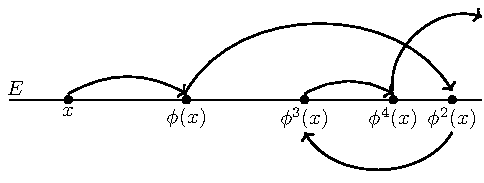
\includegraphics[width=12cm]{Tesis UNAM/graficas/sdd.pdf}
%     \caption{Evolución de $x$ bajo $\phi$ en un espacio de estados unidimensional y continuo $E$.}
%     \label{fig:evo}
% \end{figure} 

\begin{definition}
    Decimos que $x^*\in E$ es un \textbf{punto fijo} de $\phi$ si $x^*=\phi(x^*)$.
\end{definition}
\textbf{Nota:} A partir de ahora, el conjunto $E$ será un subconjunto de los números reales $\mathbb{R}$ a menos que se indique lo contrario.
\begin{definition}
\label{def:p_fijos}
    Dado un punto fijo $x^*$ de $\phi$ en un espacio de estados $E\subset\mathbb{R}$, decimos que $x^*$ es \textbf{atractor o estable} si existe un intervalo $I\subset E$ con $x^*\in I$ tal que si $y\in I$, entonces para toda $n$, se cumple $\phi^n(y)\in I$ y $\lim_{n\rightarrow\infty}\phi^n(y)=x^*$. Por otro lado, decimos que $x^*$ es \textbf{repulsor o inestable} si para toda $y\in I$ con $x^*\in I$ y $x^*\neq y$, existe un $n_{x^*}$ de forma que $\phi^{n_{x^*}}(y)\notin I$.
\end{definition}

\begin{figure}[h!]
\hfill
\subfigure[Punto fijo inestable.]{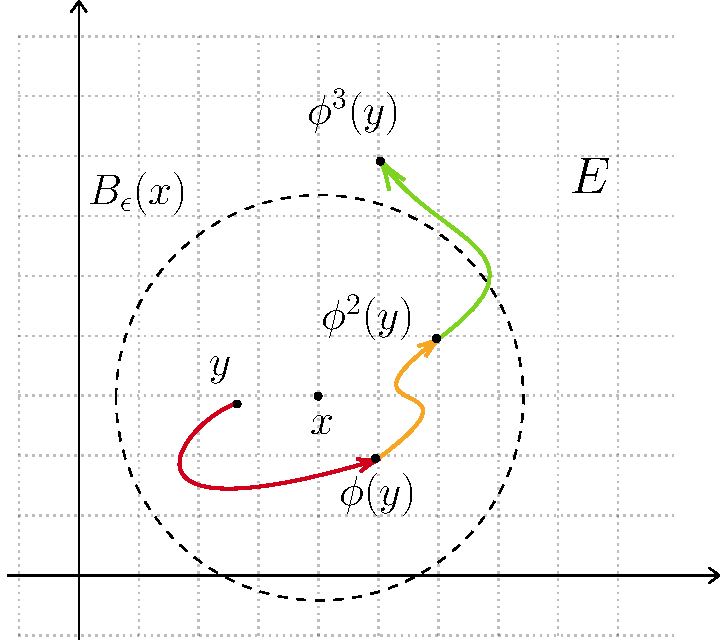
\includegraphics[width=0.49\textwidth]{Tesis UNAM/graficas/inestable.pdf}}
\hfill
\subfigure[Punto fijo estable.]{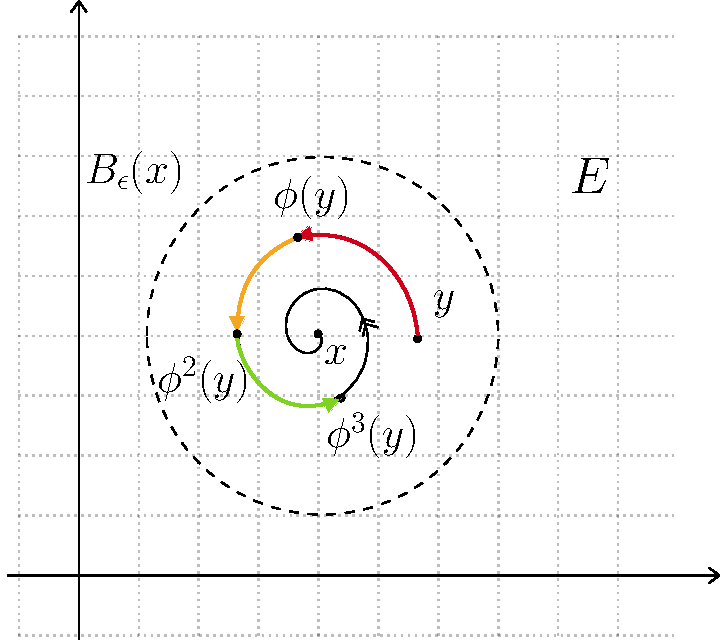
\includegraphics[width=0.49\textwidth]{Tesis UNAM/graficas/estable.pdf}}
\hfill
\caption{Ilustración de puntos fijos con diferente estabilidad en un espacio de estados $E$ bidimensional. En este caso, el intervalo $I$ de la definición \ref{def:p_fijos} es ahora una vecindad de $x$ con radio $\epsilon$ definida como $B_{\epsilon}(x)=\{z\in E: d_E(z,x)<\epsilon\}$ siendo $d$ la métrica definida en $E$.}
\label{fig:p_fijos}
\end{figure}
\begin{definition}
    Decimos que $x$ es un \textbf{punto de periodo n} de $\phi$ si $\phi^n(x)=x$ y para todo $m<n$ se tiene que $\phi^m(x)\neq x$.
\end{definition}
\begin{definition}
    Decimos que $x$ es un \textbf{punto periódico} de $\phi$ si existe $n \in \mathbb{N}$ tal que $x$ es un punto de período $n$.
\end{definition}

\begin{figure}[h!]
    \centering
    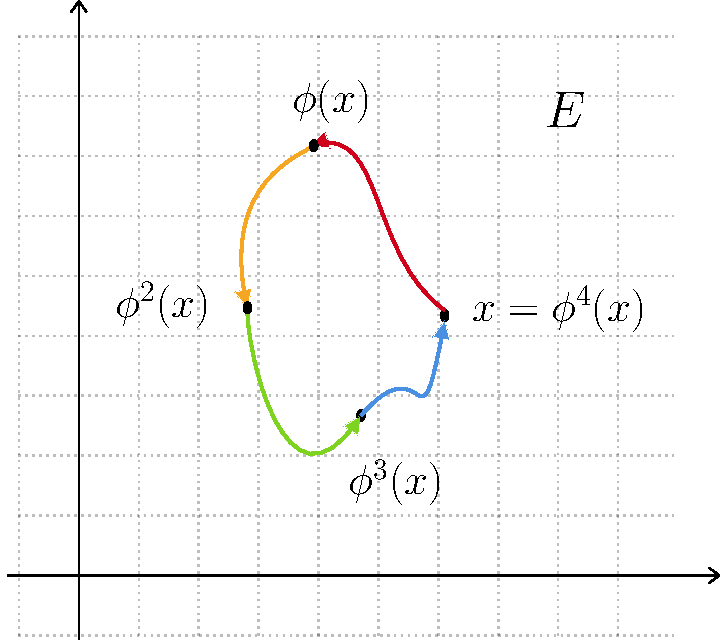
\includegraphics[width=8cm]{Tesis UNAM/graficas/periodo.pdf}
    \caption{Ilustración de un punto $x$ de periodo cuatro en un espacio de estados $E$ bidimensional.}
    \label{fig:periodo}
\end{figure} 

Los sistemas dinámicos, como los que se encuentran en biología, física y economía, suelen depender de uno o más parámetros. A medida que se varían estos parámetros, el sistema puede experimentar transiciones drásticas en su comportamiento. Estas transiciones, conocidas como bifurcaciones, son cruciales para comprender cómo los sistemas pasan de un estado estable a otro, cómo se originan patrones complejos y cómo surgen comportamientos caóticos.

\begin{definition}
    Decimos que ocurre una \textbf{bifurcación} cuando ocurre un cambio cualitativo en las orbitas del sistema. 
\end{definition}

Por ejemplo, consideremos un sistema dado por un mapeo discreto:
\[
x_{n+1} = \phi(x_n, r)
\]
donde \( r \) es un parámetro de control. A medida que \( r \) se incrementa (o disminuye), es posible que el sistema pase de un comportamiento estable a uno caótico, pasando por una serie de bifurcaciones.  Cada bifurcación corresponde a un valor crítico de \( r \) donde la naturaleza de las órbitas del sistema cambia cualitativamente.

\subsection{Caos}
    En el lenguaje natural la palabra \textit{``caos''} está asociada a desorden. Matemáticamente, un sistema caótico parece errático aun siendo determinista, pero al mismo tiempo, cumple con requisitos específicos. El primer requisito de la definición matemática contemporánea de caos recae en la idea de que una función sea sensible a las condiciones iniciales.
\begin{definition} 
    Decimos que una función $\phi$ es \textbf{sensible a condiciones inciales} en $E$ si para todo $x\in E$, existe $\epsilon >0$ tal que para todo $\delta >0$ existen $y\in E$ y $n\in \mathbb{N}$ tales que \[|x-y|<\delta \text{ y }|\phi^n(x)-\phi^n(y)|>\epsilon.\]
\end{definition}

% No hay que referenciar ahuevo, si si a Lorenz
%  Esta idea surgió en 1975 en los resultados del texto de Li y Yorke \textit{"Periodo 3 implica caos"}\cite{LiYorke1975}, donde prueban que si una función tiene un punto con período tres entonces tiene puntos con todos los períodos y además tiene un comportamiento caótico.

 En el último cuarto del siglo se fue refinando más la definición de caos con el uso de herramientas topológicas. Así, las siguientes definiciones proveen una idea más amplia de caos matemático.  
 \begin{definition}
     Decimos que un subconjunto $D$ de $E$ es \textbf{denso en $E$} si para todo subconjunto abierto $A\subset E$ se tiene que $D\cap A\neq \emptyset$
 \end{definition}
\begin{definition}
    Decimos que una función $\phi$ es \textbf{topológicamente transitiva} si para cualesquiera dos subconjuntos abiertos $A_1,A_2\subset E$, existe $x\in A_1$ y $n\in \mathbb{N}$ tales que $\phi^n(x)\in A_2$.
\end{definition}
\begin{remark}
Intuitivamente, si una función de evolución es topológicamente transitiva sobre un conjunto $E$, entonces el sistema ``recorre'' todo el conjunto $E$.
    \end{remark}
    \begin{remark}
    Si existe una órbita densa de $\phi$ en $E$, entonces $\phi$ es topológicamente transitiva\footnote{Esto no se cumple en un espacio topológico general, pero basta pedir que para todo subconjunto abierto no vacio $A\in E$ no exista un subconjunto finito y denso en $A$. Esta propiedad sí se satisface para $E\subset \mathbb{R}$, para más detalles véase \cite{Degirmenci2003}. Para las condiciones del converso, puede consultarse \cite{KingMendez2014}.}. 
\end{remark}
\begin{definition}
\label{def:caos}
    Decimos que una función $\phi:E\rightarrow E$ es una \textbf{función caótica}\cite{devaney2021} si cumple las siguientes condiciones:
    \begin{enumerate}
            \item La función $\phi$ es topológicamente transitiva.
        \item Los puntos periódicos de $\phi$ son densos en $E$.
        \item La función $\phi$ es sensible a condiciones iniciales. 
    \end{enumerate}
\end{definition}

La relación que existe entre algunas definiciones contemporáneas de caos, incluyendo las que aquí definimos, es abordada para el caso donde $E$ es un espacio métrico compacto en \cite{Aulbach2001}.


La definición \ref{def:caos} es muy general y puede ser reducida a solamente las primeras dos condiciones. 
\begin{theorem}
    Si $\phi:E\rightarrow E$ es una función topológicamente transitiva y sus puntos periódicos son densos en $E$, entonces $\phi$ es sensible a las condiciones iniciales.
\end{theorem}
Una prueba del Teorema puede ser consultada en \cite{Banks1992}.
Cuando nos restringimos a un espacio de estados como un subconjunto de los números reales, entonces se cumple el siguiente resultado: 
 \begin{theorem}
    Para todo intervalo $I\subset \mathbb{R}$ se cumple que si $\phi:I\rightarrow I$ es topológicamente transitiva, entonces sus puntos periódicos son densos en $I$.
\end{theorem}
La prueba de este Teorema puede ser consultada en \cite{Vellekoop1994}.

Un ejemplo clásico de caos es el sistema de ecuaciones de Lorenz \cite{Lorenz1963}, que modela la convección térmica en la atmósfera.
 En un sistema caótico, para ciertos valores de sus parámetros, pequeñas variaciones en la condición inicial \(x_0\) pueden llevar a trayectorias completamente diferentes, dando lugar al fenómeno coloquialmente conocido como efecto mariposa \footnote{Este término acuñado por Lorentz en su estudio de modelos meteorológicos proviene de la idea de que el aleteo de una mariposa en Brasil podría desencadenar una serie de eventos que, eventualmente, causarían un tornado en Texas.}.
 

\subsection{Ecuaciones en diferencias}
Un ejemplo de un sistema dinámico discreto son las ecuaciones en diferencias en donde la tupla $(T,E,\phi)$ de la definición \ref{def:sd} tiene como primeros elementos: $T=\mathbb{N}\text{ y }E=\mathbb{R}$.
Estos sistemas se describen mediante funciones que relacionan el estado del sistema en un instante $n$ con estados en instantes anteriores. Matemáticamente, una ecuación en diferencias de primer orden se representa como:
\[ x_{n+1} = \phi(x_n) \]
donde \(x_n\) es el estado del sistema en el tiempo \(n\) y \(\phi\) es una función que describe la evolución del sistema. 

Las ecuaciones en diferencias tienen su análogo continuo (cuando $T=\mathbb{R}$) en las ecuaciones diferenciales, las cuales se representan como:
\[\frac{d x}{dt}=\phi(x).\] 

Los sistemas dinámicos discretos tienden a exhibir comportamientos más caóticos en comparación con los sistemas continuos. Esto se debe a que los pasos discretos pueden evadir atractores que en sistemas continuos estabilizan el sistema. 
\subsubsection{Mapeo Logístico}
El mapeo logístico es uno de los sistemas dinámicos más estudiados y con muchos resultados interesantes acerca de él. La tupla que define a este sistema es $(\mathbb{N},[0,1],\phi)$, con función de evolución dada por:
\begin{equation}
\label{eq:log}
    \phi(x_n) = r x_n (1 - x_n) 
\end{equation}
donde \(r\) es un parámetro que determina el comportamiento del sistema. 

 Algunas características de este mapeo son:

\begin{itemize}
    \item Si $r<1$, el origen es el único punto fijo y es un punto fijo estable, por otro lado si $r>1$ es un punto fijo inestable.
    \item Si $1\leq r \leq 3 $, existen dos puntos fijos en el sistema: $x_1^*=0$ y $x_2^*=1-\frac{1}{r}$ los cuales se obtienen encontrando las soluciones a la ecuación \[x^* = r x^* (1 - x^*).\] el punto fijo estable\footnote{En un sistema dinámico unidimensional con $\phi$ continua no puede haber dos puntos fijos atractores consectivos, por lo que $x_1^*=0$ resulta ser un pnto fijo inestable.} es $x_2^*=\frac{r-1}{r}$.
    \item Si $3<r<4$, el mapeo logístico \ref{eq:log} tiene un comportamiento interesante concerniente al periodo de sus  bifurcaciones\footnote{El estudio de las bifurcaciones en mapeos recursivos no lineales, como el mapeo logístico, fue profundizado por Feigenbaum en 1978\cite{Feigenbaum1978}. En este texto demostró que estos sistemas presentan una estructura local de conjuntos de estabilidad de alto orden que se aproximan a una universalidad. Este fenómeno se manifiesta mediante un reescalado en bifurcaciones sucesivas, siguiendo asintóticamente una constante universal, conocida como la constante de Feigenbaum.}.

    % La sucesión de bifrcaciones en estos sistemas es la misma salvo por una constante.
    \item Si $r=4$, la función de evolución del mapeo logístico \ref{eq:log} es caótica\footnote{La prueba puede consultarse en \cite{devaney2021}.} en el intervalo [0,1], segun la definición \ref{def:caos}.
\end{itemize}
Debido a que el mapeo logístico con parámetro $r=4$ cubre todo el intervalo $[0,1]$ es un  candidato para un generador de números aleatorios en ese intervalo. 


\begin{figure}[h!]
    \centering
    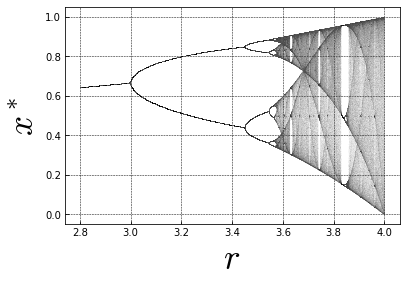
\includegraphics[width=12cm]{Tesis UNAM/graficas/Logist/Log_bif3.png}
    \caption{Diagrama de bifurcación del mapeo logístico para \( 2.8 \leq r \leq 4 \). Este diagrama muestra cómo varía el comportamiento del sistema al aumentar el parámetro \( r \). A medida que \( r \) aumenta, el sistema pasa de tener un único punto fijo estable, a experimentar duplicaciones de periodo, y finalmente a un comportamiento caótico.}
    
    \label{fig:bif-log}
\end{figure} 
\subsection{Autómatas Celulares} 


Los autómatas celulares son sistemas dinámicos discretos espaciales, en el cual el espacio de estados no es un conjunto escalar como los anteriores, sino que es una tupla, que describe la distribución espacial del sistema. El espacio es discreto, así como los valores del sistema en cada una de las posiciones espaciales, y la función de evolución $\phi$ se define para cada uno de los puntos espaciales. En los autómatas celulares, la función $\phi$ para cada punto espacial no depende de los estados de todo el espacio, sino sólo de los estados dentro de una vecindad del punto en cuestión. \\

En este trabajo usaremos los autómatas más simples,  unidimensionales. En contraste con el mapeo tienda (\ref{eq:tent}) y el mapeo logístico (\ref{eq:log}), el espacio de estados de un autómata celular unidimensional es discreto con dos estados: 0 y 1 o ``blanco'' y ``negro'' para cada punto del espacio. La forma en la que podemos visualizar la evolución del sistema será en una cuadrícula de $m\times n$, donde cada cuadro representa el estado de cierto punto espacial a cierto tiempo específico(véase la \Cref{fig:malla}). El número $m$ representa el tamaño del sistema y $n$ representa el tiempo discreto o las iteraciones de la dinámica, así que la evolución en el tiempo de este sistema unidimensional está visualizada en la malla con renglones sucesivos, empezando con una condición inicial en $E^m=\underbrace{E\times \dots \times E}_{m \text{ veces}}$, representada por el primer renglón de la cuadrícula. 

\begin{figure}[h]
\centering
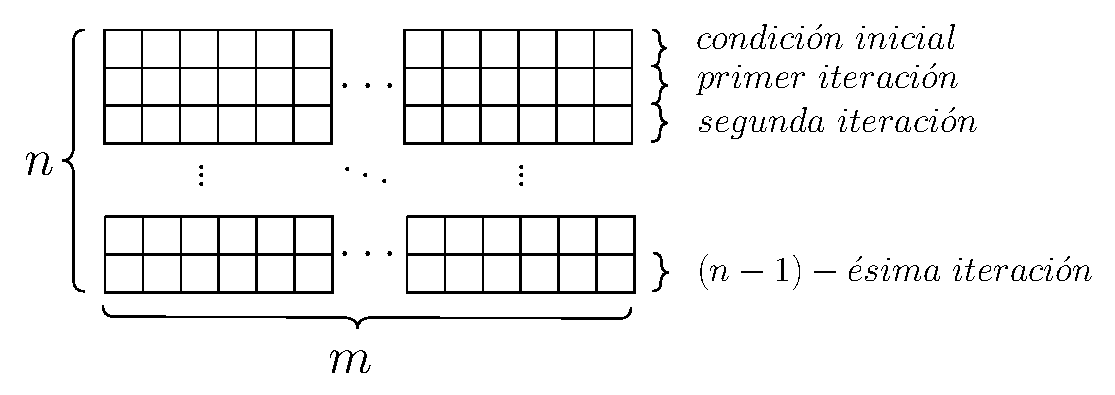
\includegraphics[width=0.8\linewidth]{Tesis UNAM/graficas/R30/Malla.pdf}
\caption{Cuadrícula donde puede ser apreciada la evolución de un automata celular unidimensional.}
\label{fig:malla}
\end{figure}

    Estos modelos son muy visuales y ayudan a modelar fenómenos cotidianos como el tránsito vehicular. Si interpretamos el primer renglón de la cuadrícula como un tramo de carretera fijo y los cuadros como espacios en donde cabe un automóvil y seguimos la idea intuitiva de que un coche puede avanzar sólo si hay espacio al frente, para hacerlo podemos modelar el comportamiento de los autos con un autómata celular unidimensional.
    
    \begin{figure}[h]
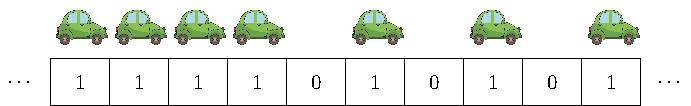
\includegraphics[width=0.95\linewidth]{Tesis UNAM/graficas/R30/regla184.pdf}
\centering
\caption{Interpretación de un renglón de la cadrícula como autos en el tráfico.}
\end{figure}

\begin{table}[h]

\centering
\begin{tabular}{@{}l|c|c|c|c|c|c|c|c@{}}
\toprule
Vecindad        &111&110&101&100&011&010&001&000\\ \midrule
Evolución $\phi$ & 1& 0& 1& 1& 1& 0& 0& 0\\ \bottomrule
\end{tabular}
\caption{Ejemplo de un posible mapeo de la función $\phi$}
\label{tab:map}
\end{table}
 Si consideramos a $\phi$ como el mapeo de vecindades expresado en la \Cref{tab:map}, tendremos un modelo de tráfico con el supuesto de que un auto solo avanza si tiene espacio al frente para hacerlo.
Otra forma de ver la función de evolución $\phi$ en la \Cref{tab:map} es un diagrama cuadricular en donde los ceros son representados con cuadros blancos y los unos con cuadros negros como el de la \Cref{fig:r128} 

\begin{figure}[h]
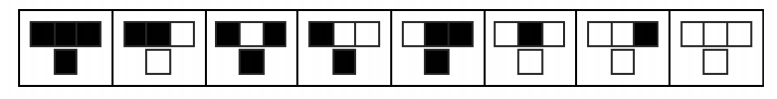
\includegraphics[width=0.8\linewidth]{Tesis UNAM/graficas/R30/184.png}
\centering
\caption{Diagrama cuadriculado de la función de evolución $\phi$ de la regla 184.}
\label{fig:r128}
\end{figure}
En cada uno de los ocho casos, la evolución del sistema (si hay o no auto en el cuadrado correspondiente en el siguiente tiempo) depende de la vecindad al tiempo anterior.
\begin{remark}
    Para cada una de las 8 posibles vecindades de un estado sólo hay dos opciones(0 ó 1), entonces existen $2^8=256$ funciones distintas $$\phi:\{0,1\}\times\{0,1\}\times\{0,1\}\rightarrow \{0,1\}.$$
     Estas distintas funciones se pueden identificar con la secuencia de unos y ceros que hay en el siguiente renglón de la tabla de evolución, para hacerlo, la secuencia completa se cambia de base dos a base 10 (decimal). En la \Cref{tab:map}, a la función de evolución $\phi$ le corresponde $10111000_2$, que en base 10 es $184$. 
\end{remark}

En la \Cref{fig:128} se ilustran tres escenarios de evolución de la regla 184. En cada uno existe un porcentaje de densidad de carros en la condición inicial: 25, 50 y 70 respectivamente. En estas mallas podemos ver cómo el comportamiento de los atascos se relega a posiciones anteriores con el paso del tiempo. 

\begin{figure}[h!]
\centering
\subfigure[Condición inicial con poca densidad de tráfico.]{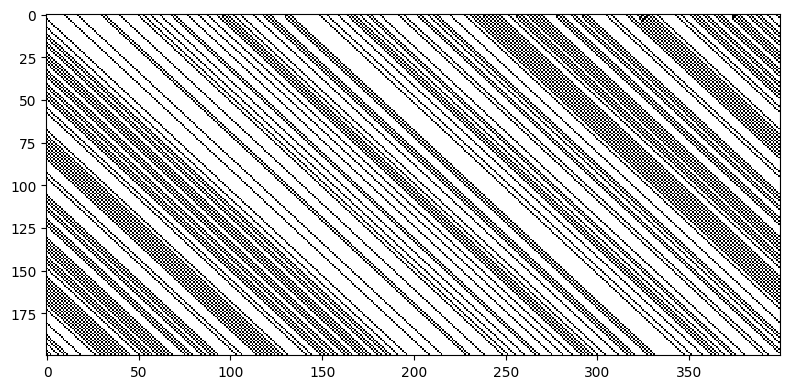
\includegraphics[width=0.7\textwidth]{Tesis UNAM/graficas/R30/Rule_184(1).png}\label{fig:sub1}}
\vfill
\subfigure[Condición inicial con densidad media de tráfico.]{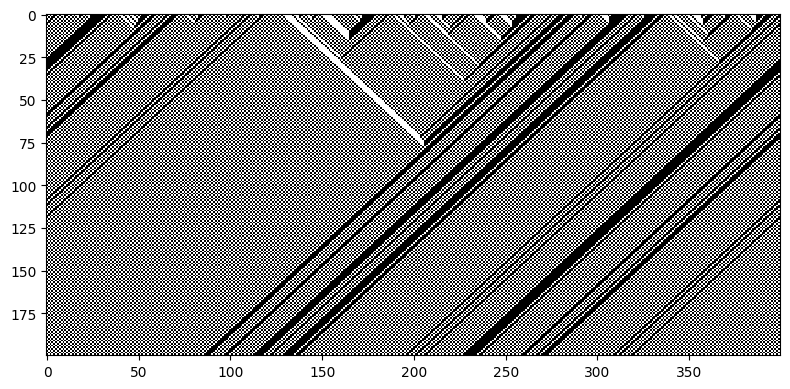
\includegraphics[width=0.7\textwidth]{Tesis UNAM/graficas/R30/Rule_184(2).png}\label{fig:sub2}}
\vfill
\subfigure[Condición inicial con densidad alta de tráfico.]{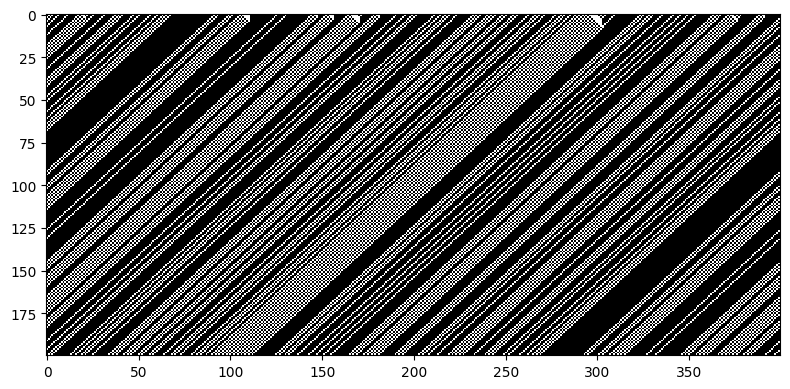
\includegraphics[width=0.7\textwidth]{Tesis UNAM/graficas/R30/Rule_184(3).png}\label{fig:sub3}}
\vfill
\caption{Regla 184 con tres condiciones iniciales diferentes.}
\label{fig:128}
\end{figure}



 
 En 1983 Wolfram publica un artículo \cite{Wolfram1983} concerniente a estos sistemas dinámicos discretos y su compleja evolución mientras intentaba replicar las redes neuronales del cerebro y otros procesos biológicos complejos. Posteriormente, en 1984 hace un estudio más detallado \cite{Wolfram2002} de uno de estos autómatas unidimensionales: la regla 30, que presenta un comportamiento muy interesante.   


\subsubsection{Regla 30}
Como ya se mencionó, la regla 30 es el sistema dinámico con función de evolución $\phi$ dada por la \Cref{tab:r30} y diagrama de evolución mostrado en la \Cref{fig:dr30}.

\begin{table}[h]
\centering
\begin{tabular}{@{}l|c|c|c|c|c|c|c|c@{}}
\toprule
Vecindad        &111&110&101&100&011&010&001&000\\ \midrule
Evolución $\phi$ & 0& 0& 0& 1& 1& 1& 1& 0\\ \bottomrule
\end{tabular}
\caption{Tabla de evolución de la regla 30.}
\label{tab:r30}
\end{table}
\begin{figure}[h]
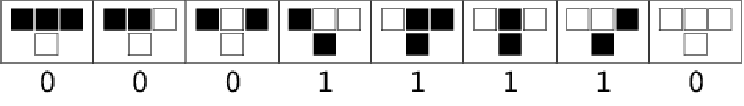
\includegraphics[width=0.8\linewidth]{Tesis UNAM/graficas/R30/Regla_30.pdf}
\centering
\caption{Diagrama cuadriculado de la función de evolución de la regla 30.}
\label{fig:dr30}
\end{figure}
El comportamiento aparentemente aleatorio de la regla 30 fue observado por Wolfram desde 1984 y en 1986 publicó un artículo sobre autómatas celulares y secuencias aleatorias \cite{wolfram1986}. Los números aleatorios obtenidos a partir del sistema dinámico de la regla 30 deben ser decodificados de la misma forma en la que se nombran las funciones, cambiando de base binaria a base decimal. Al tener una cuadrícula de $m$ columnas, tendremos a lo más el número \(\sum_{i=0}^m2^i\) que corresponde al número en binario con $m$ unos.

\begin{figure}[h!]
\hfill
\subfigure[Concha \textit{Conus textile}.]{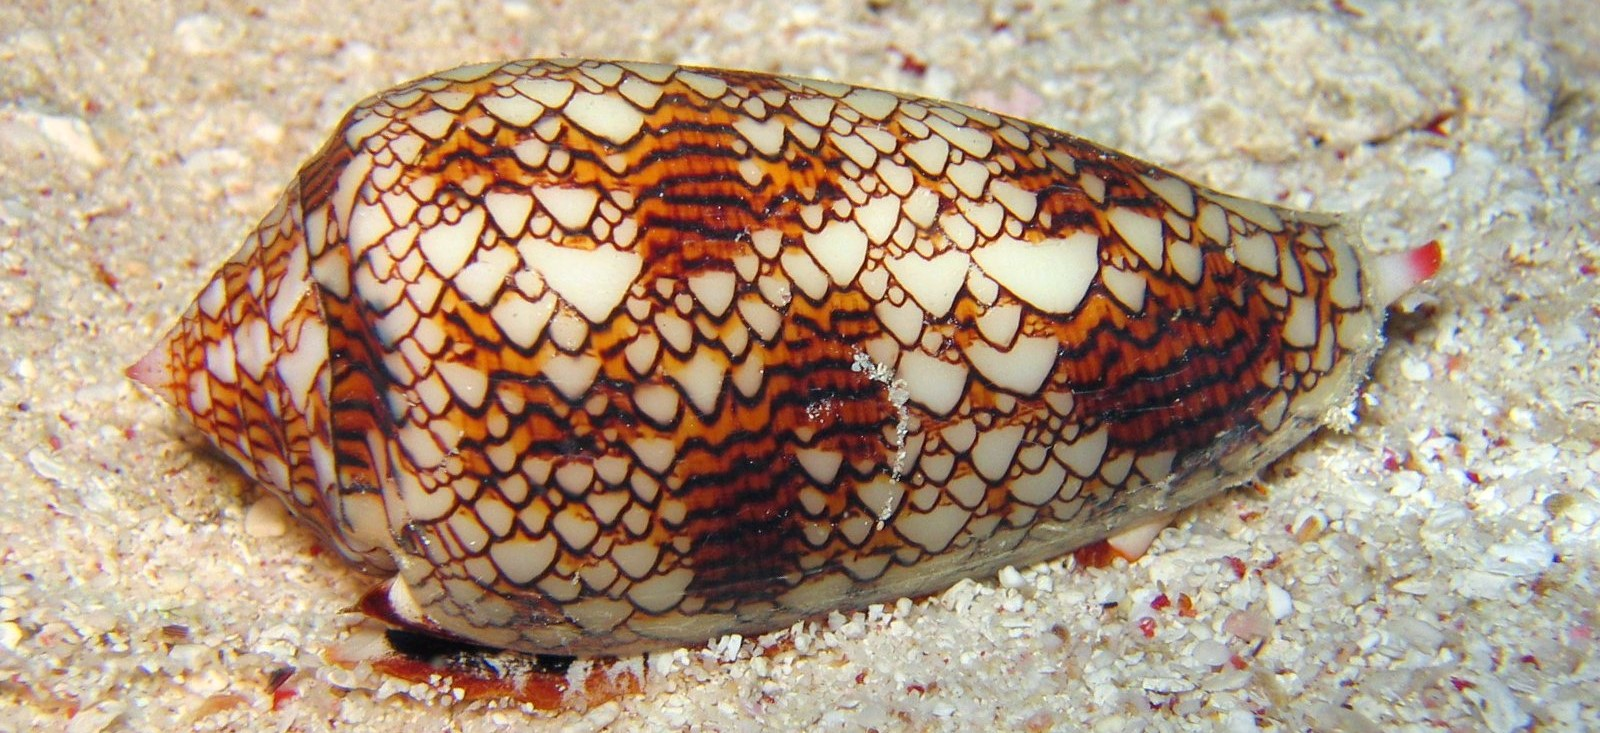
\includegraphics[width=0.53\textwidth]{Tesis UNAM/graficas/R30/Textile_cone.jpeg}}
\hfill
\subfigure[Regla 30 con 50 iteraciones.]{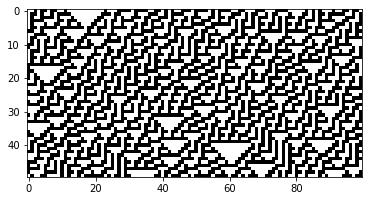
\includegraphics[width=0.45\textwidth]{Tesis UNAM/graficas/R30/regla_concha2.png}}
\hfill
\caption{Comparación entre el patrón de una concha marina y la Regla 30.}
\label{fig:R30-comp}
\end{figure}

Como se observa en la \Cref{fig:R30-comp}, los patrones caóticos generados por la Regla 30 encuentran un paralelo en la naturaleza, como se puede ver en la disposición de las marcas de la concha \textit{Conus textile}. Este tipo de comportamiento resalta cómo el caos, generado por simples reglas locales en un autómata celular, puede aparecer en estructuras biológicas.

\section{Probabilidad}
La probabilidad surge como una herramienta fundamental para describir y analizar fenómenos inciertos. Desde juegos de azar hasta modelos complejos en física, biología, economía e informática, la teoría de la probabilidad proporciona un marco matemático que permite cuantificar la incertidumbre y predecir el comportamiento de sistemas aleatorios. En esta sección se presentan los conceptos básicos que servirán como punto de partida para el estudio de números pseudoaleatorios.

\begin{definition}
El conjunto de posibles resultados de un experimento cuyo resultado es aleatorio se llama \textbf{espacio muestral} y es denotado comúnmente como $\Omega$. 
\end{definition}
Cada elemento $\omega \in \Omega$ representa un resultado elemental del experimento. 
\begin{example}
    Si se lanza una moneda, el espacio muestral es $\Omega = \{\text{águila}, \text{sol}\}$.
    \label{ej:moneda}
\end{example}
\begin{definition}
Un \textbf{evento} es cualquier subconjunto medible del espacio muestral.
\end{definition}
En el \Cref{ej:moneda}, el evento \textbf{obtener águila} es $A = \{\text{águila}\}\subset \Omega$. 
\begin{example}
    Si se lanza un dado justo, el espacio muestral es  $\Omega =\{1,2,3,4,5,6\}$ y podemos tener eventos como: \textbf{obtener un número par}, el cual sería el conjunto $$B=\{2,4,6\}\subset \Omega.$$
\end{example}
Los eventos se agrupan en una colección de subconjuntos $\mathcal{F}\subset \mathcal{P}(\Omega)=2^{\Omega}$ del espacio muestral. 

\begin{remark}
    El complemento \(B^{c}=\{1,3,5\}\) sigue siendo un evento, al igual que su unión con otros subconjuntos o su intersección con ellos.  
\end{remark}
De aquí surge la necesidad de trabajar con una colección de eventos \(\mathcal{F}\) que sea \emph{estable} ante dichas operaciones, lo que nos conduce al siguiente concepto fundamental.

Si $\mathcal{F}$ cumple que es cerrado bajo operaciones de unión, intersección y complementos, entonces es llamada $\sigma$-álgebra. Esto quiere decir que estas operaciones entre eventos siguen dando como resultado otros eventos. Lo anterior queda formalizado con la siguiente definición:

\begin{definition}
    Sea \(\Omega\) un conjunto no vacío. Decimos que una colección \(\mathcal{F}\subset 2^{\Omega}\) es una \textbf{\(\sigma\)-álgebra} sobre \(\Omega\) si cumple las tres condiciones siguientes:  

1. \(\Omega\in\mathcal{F}\);  

2. si \(A\in\mathcal{F}\), entonces su complemento \(A^{c}\in\mathcal{F}\);  

3. para toda sucesión numerable \(\{A_{n}\}_{n\in\mathbb{N}}\subset\mathcal{F}\) se tiene \(\displaystyle \bigcup_{n=1}^{\infty} A_{n}\in\mathcal{F}\).
\label{def:sigma-alg}
\end{definition}

Cuando \(\Omega\) es finito, por ejemplo: \(\{1,\dots,6\}\) en el experimento del dado, el conjunto potencia \(2^{\Omega}\) satisface las tres propiedades de la \Cref{def:sigma-alg} y, por eso, constituye una \(\sigma\)-álgebra.

% En un contexto continuo y de dinámica caótica tomamos \(\Omega=[0,1]\) y
% \[
%     \varphi:[0,1]\longrightarrow[0,1],\qquad
%     \varphi(x)=4x(1-x),
% \]
% el ya mencionado \textit{mapeo logístico} con parámetro \(r=4\).
% Trabajaremos con la \textbf{\(\sigma\)-álgebra de Borel}, denotada \(\mathcal{B}([0,1])\), la cual es la más pequeña \(\sigma\)-álgebra que contiene a todos los intervalos abiertos de \([0,1]\).
% Un evento típico en este marco es
% \[
%     A_{r}=\{\,x\in[0,1]:x<r\,\},\qquad 0<r<1,
% \]
% cuyo complemento es \(A_{r}^{c}=[r,1]\). Además, la unión de cualquier familia numerable de intervalos abiertos sigue perteneciendo a \(\mathcal{B}([0,1])\).

% La elección de \(\mathcal{B}([0,1])\) resulta natural porque:  
% \begin{enumerate}
%     \item  permite describir eventos definidos mediante condiciones sobre la órbita \(\{x_{n}\}\) generada por \(\varphi\);  

%     \item es suficientemente rica para formalizar las pruebas de uniformidad e independencia que aplicaremos más adelante.
% \end{enumerate}

Con la noción de \(\sigma\)-álgebra establecida, podemos introducir la \textit{medida de probabilidad} \(\mathbb{P}:\mathcal{F}\to[0,1]\) y enunciar las tres propiedades que debe satisfacer; estas se conocen como los \textit{axiomas de Kolmogórov} y constituyen la base del cálculo de probabilidades que emplearemos en los capítulos posteriores.

\subsection*{Axiomas de la probabilidad}
\begin{definition}

Sea \((\Omega,\mathcal F)\) un espacio medible, es decir, \(\mathcal F\) es una
\(\sigma\)-álgebra de subconjuntos de \(\Omega\).
Una aplicación
\[
    \mathbb{P}:\mathcal F \longrightarrow [0,1]
\]
se llama \textbf{medida de probabilidad} si cumple los tres postulados de Kolmogórov:

\begin{enumerate}
    \item \textbf{No–negatividad.}  
          \(\mathbb{P}(A)\ge 0\) para todo \(A\in\mathcal F\).
    \item \textbf{Normalización.}  
          \(\mathbb{P}(\Omega)=1\).
    \item \textbf{\(\sigma\)-aditividad.}  
          Para toda familia numerable de eventos disjuntos
          \(\{A_n\}_{n\in\mathbb{N}}\subset\mathcal F\),
          \[
              \mathbb{P}\!\Bigl(\,\bigcup_{n=1}^{\infty} A_n\Bigr)
              \;=\;
              \sum_{n=1}^{\infty} \mathbb{P}(A_n).
          \]
\end{enumerate}
\end{definition}
Las propiedades más habituales que se derivan inmediatamente de estos axiomas son:

\begin{itemize}
    \item [a)] \textbf{Probabilidad del vacío.}  \(\mathbb{P}(\phi) = 0\).
    \item[b)] \textbf{Complemento.}  
          \(\mathbb{P}(A^{c}) = 1 - \mathbb{P}(A)\).
    \item [c)]
    \textbf{Monotonía.}  
          Si \(A\subset B\) entonces \(\mathbb{P}(A)\le \mathbb{P}(B)\).
          \item [d)]
    \textbf{Probabilidad de la unión.}  
          \(\mathbb{P}(A\cup B) = \mathbb{P}(A)+\mathbb{P}(B)-\mathbb{P}(A\cap B)\).
    \item[e)]  \textbf{Sub–aditividad.}  
          Para cualquier familia de eventos \(\{A_n\}\),
          \(\mathbb{P}\bigl(\bigcup_{n} A_n\bigr)\le\sum_{n} \mathbb{P}(A_n)\).
    \item [f)] \textbf{Continuidad desde abajo.}  
          Si \(A_1\subset A_2\subset\dots\) y \(A=\bigcup_{n}A_n\), entonces
          \(\displaystyle \mathbb{P}(A)=\lim_{n\to\infty}\mathbb{P}(A_n)\).
    \item [g)] \textbf{Continuidad desde arriba.}  
          Si \(A_1\supset A_2\supset\dots\) y \(A=\bigcap_{n}A_n\), entonces
          \(\displaystyle \mathbb{P}(A)=\lim_{n\to\infty}\mathbb{P}(A_n)\).
\end{itemize}
Las pruebas pueden consultarse en \cite{grimmett2001probability,Ross_07}.
% \subsubsection*{Ejemplos}

% \begin{enumerate}
%     \item \textbf{Modelo de Laplace (finito).}\;  
%           Para el lanzamiento de un dado justo,
%           \(\Omega=\{1,\dots,6\}\) y \(\mathcal F=2^{\Omega}\).
%           Definiendo
%           \[
%               P(A)=\frac{|A|}{6},\qquad A\subset\Omega,
%           \]
%           se satisface cada axioma y, por tanto,
%           \((\Omega,\mathcal F,P)\) es un \emph{espacio de probabilidad}.
%     \item \textbf{Medida uniforme continua.}\;  
%           En \(\Omega=[0,1]\) con
%           \(\mathcal F=\mathcal B([0,1])\),
%           la medida de Lebesgue
%           \[
%               P(A)=\lambda(A),\qquad A\in\mathcal B([0,1]),
%           \]
%           asigna a cada intervalo su longitud y verifica los tres axiomas.
%     \item \textbf{Medida invariante del mapeo logístico.}\;  
%           Para la dinámica
%           \(\varphi(x)=4x(1-x)\),
%           existe una densidad invariante
%           \(\displaystyle f(x)=\frac{1}{\pi\sqrt{x(1-x)}}\)
%           que define la medida
%           \(P(A)=\!\int_{A} f(x)\,dx\).
%           Esta medida es absolutamente continua respecto a \(\lambda\)
%           y cumple los axiomas anteriores; además,
%           satisface \(P(\varphi^{-1}(A))=P(A)\)
%           para todo \(A\in\mathcal B([0,1])\).
% \end{enumerate}

\subsection*{Espacio de probabilidad y variable aleatoria}
\begin{definition}
Un \textbf{espacio de probabilidad} es una terna
\(
    (\Omega,\mathcal F,\mathbb{P}),
\)
donde  
\begin{enumerate}
    \item \(\Omega\) es el \textit{espacio muestral};
    \item \(\mathcal F\) es una \(\sigma\)-álgebra de subconjuntos de \(\Omega\);
    \item \(\mathbb{P}:\mathcal F\to[0,1]\) es una medida que satisface los
          axiomas de Kolmogórov.
\end{enumerate}
\end{definition}

\begin{definition}
Sea $(\Omega,\mathcal F,\mathbb{P})$ un espacio de probabilidad.
Una función $X:\Omega \to \mathbb R$ es una \textbf{variable aleatoria} si, para todo $x\in\mathbb R$, se verifica
\[
    \{\omega\in\Omega : X(\omega)\le x\}\in\mathcal F.
\]
En tal caso decimos que $X$ es \emph{$\mathcal F$-medible}.
\end{definition}
\begin{remark}
La definición anterior es equivalente a que para todo intervalo de la forma \((-\infty,x]\) se cumple
\(
    X^{-1}\bigl((-\infty,x]\bigr)\in\mathcal F.
\)
\end{remark}
La medición asigna a cada resultado elemental \(\omega\in\Omega\) un valor
real \(X(\omega)\); el comportamiento estadístico de \(X\) se describe
mediante su \emph{función de distribución acumulada} y, cuando exista,
su \emph{función de densidad}, que desarrollamos a continuación.


\subsection*{Función de distribución acumulada}

\begin{definition}
Sea $X$ una variable aleatoria sobre el espacio de probabilidad $(\Omega,\mathcal F,\mathbb{P})$.  
La \textbf{función de distribución (acumulada)} de $X$ es la aplicación
\[
    F:\mathbb R \longrightarrow [0,1], 
    \qquad 
    F(x)=\mathbb{P}\bigl(X\le x\bigr).
\]
Cuando sea necesario enfatizar el papel de la variable aleatoria,
denotaremos a la función de distribución por \(F_X\).
\end{definition}
\begin{remark}
    El evento escrito de forma explícita como
\(\{\omega\in\Omega : X(\omega)\le x\}\)
suele abreviarse simplemente por \(\{X\le x\}\).
\end{remark}

\begin{lemma}Una función de distribución \(F_X\) tiene las siguientes propiedades:
\begin{enumerate}
    \item Es monótona no decreciente.
    \item \(\displaystyle \lim_{x\to-\infty}F_X(x)=0\) y
          \(\displaystyle \lim_{x\to\infty}F_X(x)=1\).
    \item Es continua por la derecha con límite a la izquierda (càdlàg); los saltos corresponden a
          probabilidades asignadas a valores puntuales.
\end{enumerate}
\label{lemma:dist}
\end{lemma}
La prueba del \Cref{lemma:dist} puede consultarse en \cite{grimmett2001probability}.

\subsection*{Variables aleatorias discretas y continuas}

\begin{definition}
Sea $X$ una variable aleatoria sobre el espacio de probabilidad
$(\Omega,\mathcal F,P)$.
Decimos que $X$ es \textbf{discreta} si toma valores únicamente en un
subconjunto numerable $D=\{x_1,x_2,\dots\}\subset\mathbb R$.

En tal caso existe la \textbf{función de masa de probabilidad}
\[
    p_X:D\subset\mathbb R\longrightarrow[0,1],
    \qquad
    p_X(x)\;=\;\mathbb{P}(X=x),
\]

\end{definition}
\begin{remark}
    
La función de distribución acumulada de $X$ tiene saltos en cada $x_k\in D$ y es constante entre ellos.  A estas distribuciones se les denomina \emph{atómicas}.
\end{remark}
\begin{example}
\textbf{Uniforme discreta en \(\{1,2,\dots,n\}\).}\;
Sea \(X\) una variable aleatoria que toma cada valor
\(k\in\{1,\dots,n\}\) con la misma probabilidad.
La \emph{función de masa de probabilidad} es  
\[
    p_X(k)=P(X=k)=\frac{1}{n},
    \qquad k=1,\dots,n,
\]
y \(p_X(k)=0\) para \(k\notin\{1,\dots,n\}\).
La función de distribución acumulada viene dada por
\[
    F_X(x)=P(X\le x)=
    \begin{cases}
        0, & x<1,\\[4pt]
        \dfrac{\lfloor x\rfloor}{n}, & 1\le x<n,\\[10pt]
        1, & x\ge n.
    \end{cases}
\]
Obsérvese que \(F_X\) presenta saltos de tamaño \(1/n\) en cada entero.
\end{example}
\begin{example}
\textbf{Geométrica \(\operatorname{Geom}(p)\).}\;
Sea \(X\) el número de ensayos necesarios para obtener el primer éxito
en una sucesión de ensayos independientes con probabilidad
de éxito \(p\in(0,1)\).
Su \emph{función de masa de probabilidad} es
\[
    p_X(k)=P(X=k)=p(1-p)^{\,k-1},
    \qquad k\in\mathbb{N}
\]
y \(p_X(k)=0\) para \(k\le 0\).
La función de distribución acumulada viene dada por
\[
    F_X(x)=P(X\le x)=
    \begin{cases}
        0, & x<1,\\[6pt]
        1-(1-p)^{\lfloor x\rfloor}, & x\ge 1.
    \end{cases}
\]
Así, \(F_X\) presenta saltos en los enteros positivos,
con tamaños decrecientes geométricamente.
\end{example}


\begin{definition}
La variable aleatoria $X$ se llama \textbf{continua} si su función de
distribución $F_X$ puede expresarse como
\[
    F_X(x)\;=\;\int_{-\infty}^{x} f_X(u)\,du,
    \qquad x\in\mathbb R,
\]
para alguna función integrable
$f_X:\mathbb R\to[0,\infty)$
denominada \textbf{función de densidad de probabilidad}. 
En este caso $F_X$ es continua y, cuando es derivable,
cumple $f_X(x)=F'_X(x)$.
\end{definition}

\begin{lemma}Una función de densidad \(f_X\) tiene las siguientes propiedades:
\begin{enumerate}
    \item \(f_X(x)\ge 0\) para todo \(x\in\mathbb R\).
    \item \(\displaystyle \int_{-\infty}^{\infty} f_X(x)\,dx = 1\).
    \item Si \(F_X\) es diferenciable en \(x\), entonces
          \(f_X(x)=F'_X(x)\).
    \item para cualesquiera $a<b$,
\(
    P\bigl(a<X\le b\bigr)=\int_{a}^{b} f_X(t)\,dt.
\)
\end{enumerate}
\label{lemma:dens}
\end{lemma}
La prueba del \Cref{lemma:dens} puede consultarse en \cite{grimmett2001probability}.


\begin{example}
 \textbf{Uniforme continua en \((0,1)\) \(U(0,1)\).}  
          Para \(X\sim U(0,1)\),
          \[
              F_X(x)=
              \begin{cases}
                  0, & x\le 0,\\[4pt]
                  x, & 0<x<1,\\[4pt]
                  1, & x\ge 1,
              \end{cases}
              \qquad
              f_X(x)=
              \begin{cases}
                  1, & 0<x<1,\\[4pt]
                  0, & \text{en otro caso.}
              \end{cases}
          \]
          Esta es la distribución “objetivo” cuando evaluemos la uniformidad
          de los números producidos por nuestros sistemas dinámicos discretos.
\end{example}

\begin{example}
\textbf{Beta continua \(\operatorname{Beta}(\alpha,\beta)\).}\;
Sea \(X\sim \operatorname{Beta}(\alpha,\beta)\) con parámetros
\(\alpha,\beta>0\).
Su función de densidad es  
\[
    f_X(x)=\frac{1}{B(\alpha,\beta)}\,x^{\alpha-1}(1-x)^{\beta-1}=
    \frac{\Gamma(\alpha+\beta)}{\Gamma(\alpha)\Gamma(\beta)}
    \,x^{\alpha-1}(1-x)^{\beta-1},
    \qquad 0<x<1,
\]
y \(f_X(x)=0\) fuera de \((0,1)\), donde $B(\alpha,\beta)$ es la función beta,
$$
B(\alpha,\beta)=\int_{0}^{1} t^{\alpha-1}(1-t)^{\beta-1}\,dt
=\dfrac{\Gamma(\alpha)\,\Gamma(\beta)}{\Gamma(\alpha+\beta)}.
$$
 y la función gamma $\Gamma(z)$ se define para todo número real positivo $z > 0$ mediante la integral impropia:

$$
\Gamma(z) = \int_0^{\infty} t^{z-1} e^{-t} \, dt.
$$
Esta función generaliza el factorial, ya que para todo número natural $n \in \mathbb{N}$ se cumple que:
$$
\Gamma(n) = (n - 1)!.
$$
% La función de distribución se escribe mediante la función beta
% incompleta:
% \[
%     F_X(x)=I_x(\alpha,\beta)
%     =\frac{1}{B(\alpha,\beta)}
%       \int_{0}^{x} t^{\alpha-1}(1-t)^{\beta-1}\,dt,
%     \qquad 0\le x\le 1.
% \]
Un caso de interés para esta tesis es \(\operatorname{Beta}(0.5,0.5)\).
\end{example}

\begin{definition}
Sea \(X:\Omega\to\mathbb R\) una variable aleatoria en el
espacio de probabilidad \((\Omega,\mathcal F,\mathbb{P})\).
Definimos el \textbf{soporte} de \(X\) como
\[
   \operatorname{Sop}(X)
   \;=\;
   \Bigl\{x\in\mathbb R \;:\;
          \mathbb{P}\bigl(\,\{\omega\in\Omega : |X(\omega)-x|<\varepsilon\}\bigr)
          >0
          \;\text{ para todo } \varepsilon>0\Bigr\}.
\]
\end{definition}
\begin{remark}
De forma más intuitiva: El soporte son los valores que podemos “observar” al simular o medir la variable, mientras que todo lo que queda fuera ocurre con probabilidad nula, es decir, nunca los veremos en la práctica.
% Fuera del soporte, la variable toma valor con probabilidad nula, de modo que esos valores nunca se observan
%           en la práctica.
    \begin{itemize}
    \item Si \(X\) es \emph{discreta}, entonces
          \(\operatorname{Sop}(X)=\{x:\mathbb{P}(X=x)>0\}\) es también conocido como el conjunto de átomos.
    \item Si \(X\) tiene \emph{densidad} \(f_X\), el soporte es la cerradura topológica del conjunto donde \(f_X(x)>0\).

\end{itemize}

\end{remark}
% \begin{remark}
% El uso de la cerradura topológica es necesario en ciertos casos.  
% Por ejemplo, si $X \sim \operatorname{Beta}(a,b)$ con $a,b>1$, la densidad está dada por
% \[
%    f(x) \;=\; \frac{1}{B(a,b)} \, x^{a-1} (1-x)^{\,b-1}, \quad 0 < x < 1.
% \]  
% Aquí $f(x) > 0$ únicamente en el intervalo abierto $(0,1)$, pero como cualquier intervalo que contenga a $0$ o $1$ tiene probabilidad positiva, el soporte se define como la cerradura:
% \[
%    \operatorname{Sop}(X) = [0,1].
% \]
% Así, aunque $P(X=0)=P(X=1)=0$, los extremos pertenecen al soporte porque son puntos de acumulación de probabilidad.
% \end{remark}
\begin{remark}
En la distribución $\operatorname{Beta}(a,b)$ la definición del soporte como la cerradura topológica se hace evidente.  
La densidad está dada por
\[
   f(x) \;=\; \frac{1}{B(a,b)} \, x^{a-1} (1-x)^{\,b-1}, \quad 0 < x < 1.
\]

\begin{itemize}
   \item Si $a,b>1$, entonces $f(x)$ es finita y estrictamente positiva en $(0,1)$, y se anula en los extremos $0$ y $1$.  
   A pesar de que $f(0)=f(1)=0$, el soporte se toma como la cerradura
   \[
      \operatorname{Sop}(X) = [0,1],
   \]
   pues cualquier vecindad de $0$ o $1$ tiene probabilidad positiva.

   \item Si $a,b<1$, ocurre lo contrario: la densidad $f(x)$ tiende a $+\infty$ al acercarse a $0$ o a $1$, de modo que la variable se concentra cerca de los extremos.  
   Sin embargo, aun en este caso la probabilidad puntual $P(X=0)=P(X=1)=0$, y el soporte sigue siendo
   \[
      \operatorname{Sop}(X) = [0,1].
   \]
\end{itemize}

En ambos escenarios los extremos se incluyen en el soporte por ser puntos de acumulación de probabilidad.
\end{remark}

\begin{definition}
Sea $F:\mathbb R\to[0,1]$ una función de distribución acumulada.
Se define su \textbf{inversa generalizada} por
\[
    F^{-}(u)\;=\;
    \inf\bigl\{x\in\mathbb R : F(x)\ge u\bigr\},
    \qquad 0<u<1.
\]
Cuando sea necesario enfatizar la variable aleatoria,
escribiremos $F_X^{-}$.
\end{definition}

\begin{remark}
En el caso particular en que $F$ es continua y estrictamente creciente,
la inversa generalizada coincide con la inversa ordinaria \cite{BaltazarLarios2024}.
\end{remark}

\begin{lemma}
Sea $F$ la función de distribución de una variable aleatoria $X$ y
$U\sim U(0,1)$ independiente de todo lo demás.
Definamos
\[
    \tilde X \;:=\; F^{-}(U).
\]
Entonces $\tilde X$ tiene la misma distribución que $X$.
\end{lemma}

\begin{proof}
Fijemos $t\in\mathbb R$ y probemos que
\begin{equation}\label{eq:eventos}
    \{\tilde X\le t\}=\{U\le F(t)\}.
\end{equation}

\noindent\textit{($\subseteq$)\;}
Si $\tilde X\le t$, por definición de $\tilde X$ esto equivale a
$F^{-}(U)\le t$.  Dado que $F^{-}$ es no decreciente, esto implica que
para toda $\varepsilon>0$ se cumple $U\le F(t+\varepsilon)$ y,
por la continuidad por la derecha de $F$, se concluye $U\le F(t)$.

\medskip
\noindent\textit{($\supseteq$)\;}
Sea $U\le F(t)$.
Entonces $t\in\{x\in\mathbb R : F(x)\ge U\}$, lo que significa
$t\ge F^{-}(U)=\tilde X$.
Por lo tanto $\tilde X\le t$.

\medskip
La igualdad \eqref{eq:eventos} implica
\[
    P(\tilde X\le t)=P(U\le F(t))=F(t)=P(X\le t),
\]
y, como esto vale para todo $t\in\mathbb R$, concluimos que
$\tilde X$ y $X$ tienen la misma distribución.
\end{proof}

% \begin{definition}
% Sea \(F:\mathbb R\to[0,1]\) una función de distribución.
% Definimos su \textbf{inversa generalizada} como
% \[
%     F^{-1}(u)\;=\;
%     \inf\bigl\{x\in\mathbb R : F(x)\ge u\bigr\},
%     \qquad 0<u<1.
% \]
% Cuando sea necesario destacar la variable aleatoria, escribiremos
% \(F_X^{-1}\).
% \end{definition}

% \begin{lemma}
% Una función inversa generalizada \(F_X^{-1}\) tiene las siguientes propiedades:
% \begin{enumerate}
%     \item \(F_X^{-1}\) es no decreciente y \emph{casi} continua por la derecha:
%           sólo puede presentar saltos en los puntos donde \(F_X\) hace lo propio.
%     \item Si \(U\sim U(0,1)\) es independiente de todo lo demás, entonces
%           \[
%               X := F_X^{-1}(U)
%               \quad\Longrightarrow\quad
%               P(X\le x)=F_X(x)\;\;\text{ para todo }x\in\mathbb R.
%           \]
%           Es decir, \(X\) \textbf{tiene distribución \(F\)}, incluso cuando
%           \(F\) no es estrictamente creciente.
%     \item Si \(F\) es estrictamente creciente y continua,
%           la fórmula anterior coincide con la inversa clásica:
%           \(F^{-1}(u)=\min\{x:F(x)=u\}\).
% \end{enumerate}
% \end{lemma}
%-------------------------------------------------

%-------------------------------------------------
\subsection*{Principio de inclusión–exclusión}
%-------------------------------------------------

El principio de inclusión–exclusión (P.I.E.) permite calcular la
probabilidad de la unión de varios eventos (no necesariamente disjuntos) corrigiendo los
\emph{sobrecuentos} producidos por las intersecciones.

\begin{proposition}
Sean $A_1,\dots,A_n\in\mathcal F$ eventos en un espacio de probabilidad
$(\Omega,\mathcal F,P)$. Entonces
\begin{equation}
\begin{aligned}
P\!\Bigl(\bigcup_{i=1}^{n} A_i\Bigr)
  &=\;
    \sum_{i=1}^{n} P(A_i)
    - \sum_{1\le i_1<i_2\le n} P(A_{i_1}\cap A_{i_2}) \\
  &\quad
    + \sum_{1\le i_1<i_2<i_3\le n} P(A_{i_1}\cap A_{i_2}\cap A_{i_3})
    -\; \cdots
    + (-1)^{n+1} P\Bigl(\bigcap_{i=1}^{n} A_i\Bigr).
\end{aligned}
\label{eq:pie1}
\end{equation}

\end{proposition}

\begin{proof}
La demostración es por inducción en el número \(n\) de eventos.

% \noindent\textbf{Caso base \(n=2\).}
% La fórmula se reduce a
% \[
%    P(A_1\cup A_2)=P(A_1)+P(A_2)-P(A_1\cap A_2),
% \]
% lo cual se puede deducir de los axiomas de la probabilidad observando que los conjuntos $A\cup B\text{ y } B$ se pueden descomponer en conjuntos disjuntos de la siguiente manera: $$A∪B=A∪(B∖A)\text{ y  }B=(B∖A)∪(A∩B).$$ 

\noindent\textbf{Caso base \(n=2\).}  
La fórmula se reduce a
\[
   P(A_1\cup A_2)=P(A_1)+P(A_2)-P(A_1\cap A_2).
\]
En efecto, nótese que
\[
A_1\cup A_2 = A_1 \cup (A_2\setminus A_1), \qquad   
A_2 = (A_2\setminus A_1)\cup (A_1\cap A_2),
\]
donde las uniones son disjuntas.  
Por la aditividad finita de la probabilidad se tiene
\[
P(A_1\cup A_2) = P(A_1) + P(A_2\setminus A_1).
\]
Sustituyendo
\[
P(A_2) = P(A_2\setminus A_1) + P(A_1\cap A_2),
\]
obtenemos
\[
P(A_1\cup A_2) = P(A_1) + P(A_2) - P(A_1\cap A_2),
\]
que coincide con la fórmula en el caso base.

\noindent\textbf{Hipótesis inductiva.}
Supongamos que para un cierto \(n\ge 2\) se cumple la \Cref{eq:pie1}.
% \begin{equation}
%    P\!\Bigl(\bigcup_{i=1}^{n} A_i\Bigr)
%    \;=\;
%    \sum_{r=1}^{n} (-1)^{r+1}
%    \!\!\!
%    \sum_{1\le i_1<\dots<i_r\le n}
%    \!\!\!\!\!
%      P(A_{i_1}\cap\dots\cap A_{i_r}).
%      \label{eq:pie2}
% \end{equation}

% \begin{remark}
%     Definimos
% \[
%    S_r \;:=\!
%    \sum_{1\le i_1<i_2<\dots<i_r\le n}
%    P\!\bigl(A_{i_1}\cap A_{i_2}\cap\dots\cap A_{i_r}\bigr).
% \]
% Entonces la igualdad \ref{eq:pie2} se reescribe como:
% \begin{align*}
%    P\!\Bigl(\bigcup_{i=1}^{n}A_i\Bigr)
%    \;&=\;
%    \sum_{r=1}^{n} (-1)^{r+1}\,S_r\\
%    &=\;
%    (+)\,S_1
%    \;-\;
%    S_2
%    \;+\;
%    S_3
%    \;-\;\cdots
%    +(-1)^{n+1}S_n,\\
%    &=\;
%     \sum_{k=1}^{n} P(A_k)
%     - \sum_{1\le i<j\le n} P(A_i\cap A_j) \\
%   &\quad
%     + \sum_{1\le i<j<\ell\le n} P(A_i\cap A_j\cap A_\ell)
%     -\; \cdots
%     + (-1)^{n+1} P\Bigl(\bigcap_{k=1}^{n} A_k\Bigr).
% \end{align*}
% \end{remark}

El objetivo es demostrar que la fórmula también vale para \(n+1\) eventos
\(A_1,\dots,A_{n+1}\). Para eso usaremos la estrategia donde separamos el último evento \(A_{n+1}\) de forma similar al caso base:
\begin{equation}
\begin{aligned}
   P\!\Bigl(\bigcup_{i=1}^{n+1}A_i\Bigr)
   &=
   P\!\Bigl(\bigcup_{i=1}^{n}A_i\Bigr)
   +P(A_{n+1})
   -P\!\Bigl(\bigl(\bigcup_{i=1}^{n}A_i\bigr)\cap A_{n+1}\Bigr). 
   \label{eq:pie-sep}
\end{aligned}
\end{equation}
Si consideramos \(B_i := A_i\cap A_{n+1}\) para \(i\in\{1,\dots, n\}\), entonces
\[
  \bigl(\bigcup_{i=1}^{n}A_i\bigr)\cap A_{n+1} = \bigcup_{i=1}^{n}B_i,.
\]
Los conjuntos \(B_1,\dots,B_n\) son \(n\) eventos y, por la hipótesis inductiva, satisfacen el P.I.E. 
\begin{equation}
\begin{aligned}
P\!\Bigl(\bigcup_{i=1}^{n} B_i\Bigr)
  &=\;
    \sum_{i=1}^{n} P(B_i)
    - \sum_{1\le i_1<i_2\le n} P(B_{i_1}\cap B_{i_2}) \\
  &\quad
    + \sum_{1\le i_1<i_2<i_3\le n} P(B_{i_1}\cap B_{i_2}\cap B_{i_3})
    -\; \cdots\\
  &\quad+ (-1)^{n+1} P\Bigl(\bigcap_{i=1}^{n} B_i\Bigr).
\end{aligned}
\label{PIEv2}
\end{equation}
También observemos que para cualesquiera eventos $B_{i_1},\dots,B_{i_r}\in\mathcal F$ con \(r\in\{1,\dots, n\}\)
\[
  B_{i_1}\cap\dots\cap B_{i_r}
  =
  (A_{i_1}\cap\dots\cap A_{i_r})\cap A_{n+1},
\]
de modo que
\[
   P(B_{i_1}\cap\dots\cap B_{i_r})
   =
   P(A_{i_1}\cap\dots\cap A_{i_r}\cap A_{n+1}).
\]
Así la \Cref{PIEv2} puede reescribirse como
\begin{equation}
\begin{aligned}
P\!\Bigl(\bigcup_{i=1}^{n} B_i\Bigr)
  &=\;
    \sum_{i=1}^{n} P(A_i\cap A_{n+1})
    - \sum_{1\le i_1<i_2\le n} P(A_{i_1}\cap A_{i_2}\cap A_{n+1}) \\
  &\quad
    + \sum_{1\le i_1<i_2<i_3\le n} P(A_{i_1}\cap A_{i_2}\cap B_{i_3}\cap A_{n+1})
    -\; \cdots\\
  &\quad+ (-1)^{n+1} P\Bigl(\bigcap_{i=1}^{n} A_i\cap A_{n+1}\Bigr).
\end{aligned}
\label{PIEv3}
\end{equation}
 Sustituyendo en la descomposición inicial \ref{eq:pie-sep} tenemos:
\begin{equation}
\begin{aligned}
   P\!\Bigl(\bigcup_{i=1}^{n+1}A_i\Bigr)
   &=
   \underbrace{P\!\Bigl(\bigcup_{i=1}^{n}A_i\Bigr)}_{\text{(i)}}
   +\underbrace{P(A_{n+1})}_{\text{(ii)}}
   -\underbrace{P\!\Bigl(\bigcup_{i=1}^{n}B_i\Bigr)}_{\text{(iii)}}.
\end{aligned}
\label{eq:aux}
\end{equation}

\noindent\textbf{(i)}
Por la hipótesis inductiva,  
\begin{equation}
\begin{aligned}
P\!\Bigl(\bigcup_{i=1}^{n} A_i\Bigr)
  &=\;
    \sum_{i=1}^{n} P(A_i)
    - \sum_{1\le i_1<i_2\le n} P(A_{i_1}\cap A_{i_2}) \\
  &\quad
    + \sum_{1\le i_1<i_2<i_3\le n} P(A_{i_1}\cap A_{i_2}\cap A_{i_3})
    -\; \cdots
    + (-1)^{n+1} P\Bigl(\bigcap_{i=1}^{n} A_i\Bigr).
\end{aligned}
\end{equation}

\noindent\textbf{(ii)} El término \(P(A_{n+1})\) se puede agregar al primer sumando de forma que

\begin{equation}
\begin{aligned}
\textbf{(i)}+\textbf{(ii)}
  &=\;
    \sum_{i=1}^{n+1} P(A_i)
    - \sum_{1\le i_1<i_2\le n} P(A_{i_1}\cap A_{i_2}) \\
  &\quad
    + \sum_{1\le i_1<i_2<i_3\le n} P(A_{i_1}\cap A_{i_2}\cap A_{i_3})
    -\; \cdots
    + (-1)^{n+1} P\Bigl(\bigcap_{i=1}^{n} A_i\Bigr).
\end{aligned}
\label{eq:aux2}
\end{equation}
\noindent\textbf{(iii)}Al sustraer el término \(P\!\Bigl(\bigcup_{i=1}^{n}B_i\Bigr)\) en la \Cref{eq:aux}, todos los sumandos de la \Cref{PIEv3} cambian de signo y se pueden sumar con los términos de \ref{eq:aux2} a partir del segundo sumando.

Así, al reunir todos los términos individuales $\textbf{(i)},\textbf{(ii)},\textbf{(iii)}$ se obtiene
\begin{equation}
\begin{aligned}
P\!\Bigl(\bigcup_{i=1}^{n+1} A_i\Bigr)
  &=\;
    \sum_{i=1}^{n+1} P(A_i)
    - \sum_{1\le i_1<i_2\le n+1} P(A_{i_1}\cap A_{i_2}) \\
  &\quad
    + \sum_{1\le i_1<i_2<i_3\le n+1} P(A_{i_1}\cap A_{i_2}\cap A_{i_3})
    -\; \cdots
    + (-1)^{(n+1)+1} P\Bigl(\bigcap_{i=1}^{n+1} A_i\Bigr).
\end{aligned}
\end{equation}
lo que demuestra la validez de la fórmula para \(n+1\).
Por inducción, la proposición es cierta para todo \(n\ge 2\).
\end{proof}

Con el principio de inclusión–exclusión completamos el conjunto de
herramientas probabilísticas básicas necesarias para el análisis de los generadores pseudoaleatorios construidos a partir de
sistemas dinámicos caóticos.


\subsection{Números Pseudoaleatorios}

Recordemos que los números pseudoaleatorios son aquellos generados por un algoritmo determinista y que tienen propiedades estadísticas que los hacen indistinguibles de los números verdaderamente aleatorios. En la simulación de números pseudoaleatorios, la generación de variables uniformes en el intervalo $[0,1]$ es sumamente importante, pues a partir de ellas podemos generar otras distribuciones. Si queremos simular una variable aleatoria $X$ con función de distribución $F_X$, definimos \[Y=F^{-1}_X(U)\text{  donde   }U\sim \mathrm{Uniforme}[0,1]\] 
% \begin{remark} Mucho desmadre
%     La función de distribución $F_X$ es una función continua e inyectiva cuyo contradominio es el intervalo $[0,1]$, por lo que la variable $Y$ está bien definida.
% \end{remark}

Calculando la función de densidad de $Y$ obtenemos
\[F_Y(y)=P(Y\leq y)=P(U\leq F(y))=F(y)\] debido a que la densidad uniforme se define como:
\[f_X(y)=\mathbf{1}_{[0,1]}(y).\] 
Concluyendo que $Y$ tiene función de densidad $F_X$, es decir, $Y\sim X$.
\begin{remark}
    No siempre se puede hacer esta técnica para generar distribuciones, pues la función inversa de la densidad no se puede escribir explícitamente para todas las variables aleatorias.
\end{remark}
Otro resultado muy parecido que también es relevante para este trabajo es el siguiente. 
\begin{proposition}
\label{prop:inv}
    Si $X$ es una variable aleatoria continua, entonces se cumple que \[F_X(X)\sim Unif(0,1)\]
\end{proposition}
\begin{proof}
Si consideramos \[U=F_X(X)\] y calculamos $F_U(x)$ obtenemos
    \[F_U(x)=P(U\leq x) = P(F_X(X)\leq x) \]
    como $F$ es una función monótona creciente y continua en $[0,1]$ podemos invertir la función 
    \[F_U(x)= P(X\leq F^{-1}_X(x))=F_X(F^{-1}_x(x))=x \cdot \mathbf{1}_{[0,1]}(x)\] y por lo tanto  \[F_X(X)\sim Unif(0,1).\]
\end{proof}
\subsection{Propiedades de los Números Pseudoaleatorios}

Como ya mencionamos, para que una sucesión de números generados por un algoritmo determinista pueda denominarse pseudoaleatoria debe cumplir con ciertas características. En esta sección abordaremos las propiedades que estas sucesiones deben cumplir y las herramientas matemáticas que se utilizan para verificarlas. 
\subsubsection{Uniformidad}
La uniformidad es una propiedad deseada en la generación de números pseudoaleatorios, ya que indica que los números están distribuidos uniformemente en el intervalo [0, 1]. Esta propiedad puede evaluarse mediante histogramas, momentos y la función generadora de momentos.

\subsubsection{Independencia}
% La independencia es otra propiedad importante, ya que de ella derivan otras propiedades que son muy útiles en la aplicación de las simulaciones en otras áreas de conocimiento. 

La independencia es una de las propiedades fundamentales en probabilidad y juega un papel central en la simulación. En términos generales, dos eventos son independientes cuando la ocurrencia de uno no afecta la probabilidad de ocurrencia del otro.  

En simulaciones, esta propiedad es esencial porque permite interpretar cada muestra como una réplica imparcial del experimento. Si las realizaciones no fueran independientes, aparecerían correlaciones que alterarían los resultados, produciendo estimaciones sesgadas y reduciendo la validez estadística de los métodos.  

\begin{definition}
    Definimos a la \textbf{probabilidad condicional} de la variable $X$ dada la variable $Y$ como \[P(X|Y)=\frac{P(X\cap Y)}{P(Y)}\]
\end{definition}
\begin{definition}
\label{def:ind}
    Decimos que dos variables aleatorias $X,Y$ son \textbf{independientes} si la probabilidad condicional de $X$ dada $Y$ es simplemente la probabilidad de $X$, es decir, \[P(X|Y)=P(X)\]
\end{definition}

De la definición \ref{def:ind} podemos deducir que la independencia de variables aleatorias implica \[P(X\cap Y)=P(X)P(Y)\]
La independencia de un conjunto de datos es importante para evitar sesgos en los resultados de experimentos realizados con esos datos. Podemos tener un conjunto de datos obtenidos de una misma distribución pero que no sean independientes. No obstante, si ya contamos con un conjunto de datos provenientes de una distribución de interés, existen técnicas simples para dotar de independencia al conjunto de datos. 

% \textcolor{red}{Explicar que un reordenamiento de los datos puede mejorar los resultados de independencia.}
\subsection{Métodos de Evaluación }

En esta subsección abordaremos las herramientas para cotejar los números pseudoaleatorios generados en este trabajo.
\subsubsection{Histograma}

Un \textbf{histograma} es una representación gráfica de la densidad de probabilidad de un conjunto de datos. En un histograma, el eje horizontal representa los intervalos de datos, mientras que el eje vertical indica la frecuencia de aparición o densidad de los datos dentro de cada intervalo.

Los histogramas se utilizan para:

\begin{itemize}
    \item \textbf{Visualizar la Distribución de los Datos}: Permiten observar cómo se distribuyen los datos en un rango específico. Es útil para identificar patrones como simetría, asimetría, y la presencia de colas pesadas.
    \item \textbf{Detección de Anomalías}: Ayudan a identificar la presencia de datos atípicos (outliers).
    \item \textbf{Comparación de Distribuciones}: Facilitan la comparación visual de diferentes conjuntos de datos o modelos teóricos, como la comparación entre la distribución empírica de los datos y una función de densidad teórica.
\end{itemize}

Para visualizar todas estas características se ilustran los histogramas de una distribución Normal y una distribución Cauchy en la \Cref{fig:hist}.
\begin{figure}[h!]
\centering
\subfigure[Histograma de datos normales comparados con la función de densidad de una variable aleatoria Normal.\label{fig:hist_norm}]{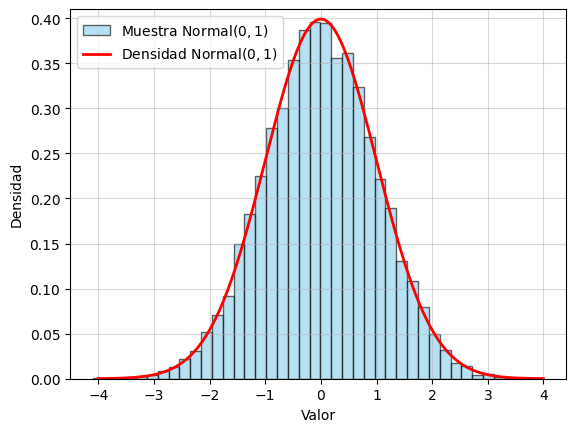
\includegraphics[width=0.49\textwidth]{Tesis UNAM/graficas/hist_norm.png}}
\hfill
\subfigure[Histograma de datos provenientes de una distribución Cauchy comparados con la función de densidad de una variable aleatoria Cauchy.\label{fig:hist_cauch}]{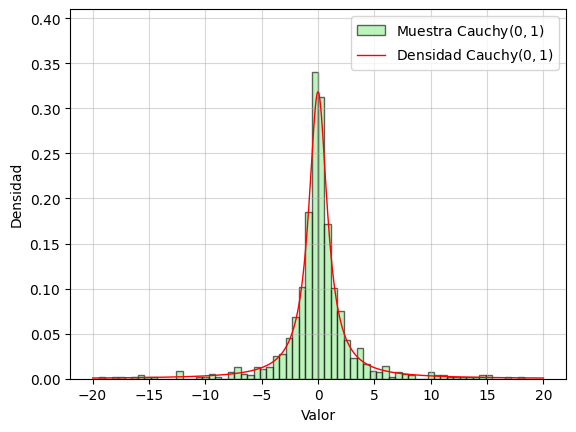
\includegraphics[width=0.49\textwidth]{Tesis UNAM/graficas/hist_cauch.png}}
\caption{Comparación entre histogramas de una variable Normal y una variable Cauchy.}
\label{fig:hist}
\end{figure}


En el histograma de la distribución normal(figura \ref{fig:hist_norm}), los datos se agrupan alrededor de la media (en este caso, cero), con una simetría evidente y una rápida disminución en las frecuencias conforme se alejan de la media. Las barras son más altas en el centro y descienden uniformemente hacia los lados. Esto se puede interpretar como:
\begin{itemize}
    \item \textbf{Centro}: La mayor parte de los datos se encuentran cerca de la media, indicando que los valores centrales son los más frecuentes.
    \item \textbf{Simetría}: La simetría alrededor de la media sugiere una distribución equilibrada de los datos.
    \item \textbf{Colas}: Las colas del histograma (las barras más alejadas del centro) son delgadas, indicando que los valores extremos son menos comunes.
\end{itemize}
 La curva de la función de densidad normal superpuesta al histograma muestra cómo se espera que se distribuyan los datos en una distribución normal. La concordancia entre el histograma y la curva indica que los datos siguen aproximadamente una distribución normal.

En el histograma de la distribución Cauchy(figra \ref{fig:hist_cauch}), se observa una concentración central similar, pero con una notable diferencia en las colas, que son mucho más gruesas en comparación con la distribución normal. Esto se puede interpretar como:
\begin{itemize}
    \item \textbf{Centro}: Al igual que la normal, los datos se agrupan alrededor de un punto central (en este caso, cero).
       \item \textbf{Simetría}: La simetría alrededor de la media sugiere al igual que en la distribución Normal, una distribución balanceada de los datos.
    \item \textbf{Colas}: A diferencia de la distribución normal, la distribución Cauchy tiene colas mucho más pesadas, lo que indica una mayor probabilidad de ocurrencia de valores extremos.
    % \item \textbf{Inexistencia de Momentos}: Las colas pesadas también implican que los momentos (como la media y la varianza) no están definidos, lo cual es característico de la distribución Cauchy.
\end{itemize}

 La comparación del histograma con la curva de densidad proporciona una visualización intuitiva de la distribución de los datos, facilitando la comprensión de su naturaleza. Estas características hacen de los histogramas una herramienta esencial para explorar y analizar datos.

\subsubsection{Momentos}
Los momentos de una variable aleatoria son cantidades relevantes en la distribución de una variable aleatoria que describen sus características estadísticas. 
\begin{definition}
    El \textbf{n-ésimo momento} de una \textbf{variable aleatoria discreta} \( X \) con función de masa de probabilidad \( p(x) \) está dado por:

\[
\mu_n = \mathbb{E}[X^n] = \sum_{x\in Sop_X} x^n p(x)
\]

donde \( \mathbb{E}[X^n] \) representa la esperanza de \( X^n \).
\end{definition}
\begin{definition}
    El \textbf{n-ésimo momento} de una \textbf{variable aleatoria continua} \( X \) con función de densidad de probabilidad \( f(x) \) está dado por:

\[
\mu_n = \mathbb{E}[X^n] = \int_{-\infty}^{\infty} x^n f(x) \, dx
\]

donde \( \mathbb{E}[X^n] \) representa la esperanza de \( X^n \).
\end{definition}

\textbf{Primer Momento (Media)}

El primer momento de una distribución, también conocido como la \textbf{media}, está dado por:

\[
\mu_1 = \mathbb{E}[X] = \begin{cases}
\sum_{x} x p(x) & \text{(variable discreta)} \\
\int_{-\infty}^{\infty} x f(x) \, dx & \text{(variable continua)}
\end{cases}
\]
Este momento describe el centro de masa de la distribución.

\textbf{Segundo Momento (Varianza)}

El segundo momento centralizado se conoce como la \textbf{varianza} y se calcula como:

\[
\text{Var}(X) = \mathbb{E}[(X - \mathbb{E}[X])^2] = \begin{cases}
\sum_{x} (x - \mu_1)^2 p(x) & \text{(variable discreta)} \\
\int_{-\infty}^{\infty} (x - \mu_1)^2 f(x) \, dx & \text{(variable continua)}
\end{cases}
\]
Este momento describe la dispersión de la distribución alrededor de la media.

\textbf{Tercer Momento (Asimetría)}

El tercer momento centralizado mide la \textbf{asimetría} de la distribución:

\[
\text{Asimetría} = \mathbb{E}\left[\left(\frac{X - \mu_1}{\sigma}\right)^3\right]
\]

donde \(\sigma = \sqrt{\text{Var}(X)}\) es la desviación estándar de \(X\).
Este momento describe la falta de simetría de la distribución.

\textbf{Cuarto Momento (Curtosis)}

El cuarto momento centralizado mide la \textbf{curtosis}, que es una medida asociada a la cantidad de valores en las colas o valores anormales(outliers) de la distribución:

\[
\text{Curtosis} = \mathbb{E}\left[\left(\frac{X - \mu_1}{\sigma}\right)^4\right]
\]

Comparar los momentos de los números generados numéricamente con sus contrapartes teóricas es una herramienta eficaz para evaluar la calidad y uniformidad de los datos simulados. Sin embargo, el \textit{problema de los momentos} \cite{akhiezer2021,shohat1970,schmudgen2017} revela que, aunque útil, esta técnica tiene limitaciones, ya que no siempre es posible reconstruir una distribución completa a partir de sus momentos. Por lo tanto, esta evaluación, aunque valiosa, no garantiza una representación exacta de la distribución.


\subsubsection{Función Generadora de Momentos}
% La FGM encapsula todos los momentos de una distribución y es útil para analizar la calidad de los números generados.
La función generadora de momentos (FGM) de una variable aleatoria es una herramienta importante en teoría de probabilidad y estadística, utilizada para caracterizar la distribución de una variable aleatoria.
\begin{definition}
    Si \( X \) es una variable aleatoria discreta con función de masa de probabilidad \( p(x) \), la \textbf{función generadora de momentos} \( M_X(t) \) está definida como:

\[
M_X(t) = \mathbb{E}[e^{tX}] = \sum_{x\in Sop_X} e^{tx} p(x)
\]

donde la suma es sobre todos los valores posibles de \( X \).
\end{definition}
\begin{definition}
    Si \( X \) es una variable aleatoria continua con función de densidad de probabilidad \( f(x) \), la \textbf{función generadora de momentos} \( M_X(t) \) se define como:

\[
M_X(t) = \mathbb{E}[e^{tX}] = \int_{-\infty}^{\infty} e^{tx} f(x) \, dx
\]
\end{definition}


\textbf{Propiedades de la Función Generadora de Momentos}

1. \textbf{Existencia}: La FGM \( M_X(t) \) existe si la esperanza \( \mathbb{E}[e^{tX}] \) es finita para algún intervalo de valores de \( t \) alrededor de 0.

2. \textbf{Relación con los Momentos}: Los momentos de una variable aleatoria \( X \) pueden obtenerse derivando la FGM. Específicamente, el $n$-ésimo momento de \( X \) está dado por:
   \[
   \mathbb{E}[X^n] = M_X^{(n)}(0)
   \]
   donde \( M_X^{(n)}(t) \) denota la $n$-ésima derivada de \( M_X(t) \) con respecto a \( t \).

3. \textbf{Caracterización de la Distribución}: La FGM \( M_X(t) \), si existe en un intervalo abierto alrededor de cero, determina de manera única la distribución de la variable aleatoria \( X \).

Estos resultados pueden ser consultados en \cite{GVK164761632,Ross_07,billingsley1995probability}.

\begin{example}
    
\textbf{Distribución Normal}

Para una variable aleatoria \( X \) con distribución normal \( \mathcal{N}(\mu, \sigma^2) \), la FGM está dada por:

\[
M_X(t) = \exp\left(\mu t + \frac{\sigma^2 t^2}{2}\right)
\]
\end{example}

\begin{example}
\textbf{Distribución Cauchy}

Una variable aleatoria \( X \) tiene una distribución Cauchy con parámetros de ubicación \( x_0 \) y escala \( \gamma \) si su función de densidad de probabilidad está dada por:

\[
f_X(x) = \frac{1}{\pi \gamma \left[ 1 + \left( \frac{x - x_0}{\gamma} \right)^2 \right]}
\]

donde \( x_0 \) es el parámetro de ubicación y \( \gamma > 0 \) es el parámetro de escala.

% \textbf{Función Generadora de Momentos}
La FGM de la distribución Cauchy es:

\[
M_X(t) = \mathbb{E}[e^{tX}] = \int_{-\infty}^{\infty} e^{tx} f_X(x) \, dx = \int_{-\infty}^{\infty} e^{tx} \frac{1}{\pi \gamma \left[ 1 + \left( \frac{x - x_0}{\gamma} \right)^2 \right]} \, dx
\]
\end{example}


% \[
% M_X(t) = \int_{-\infty}^{\infty} e^{tx} \frac{1}{\pi \gamma \left[ 1 + \left( \frac{x - x_0}{\gamma} \right)^2 \right]} \, dx
% \]

% \textbf{Inexistencia de la FGM}

Para la distribución Cauchy, la integral anterior no converge para ningún \( t \neq 0 \). Esto se debe a que, para valores grandes de \( |x| \), el término \( e^{tx} \) crece exponencialmente mientras que la función de densidad decae solo como \( \frac{1}{x^2} \). La función \( f_X(x) \) no decrece lo suficientemente rápido para contrarrestar el crecimiento de \( e^{tx} \) cuando \( |x| \to \infty \).

La esperanza \(\mathbb{E}[e^{tX}]\) diverge, lo que significa que la FGM \( M_X(t) \) no está finitamente definida para ningún \( t \neq 0 \). Por tanto, \textbf{la función generadora de momentos para una variable aleatoria con distribución Cauchy no existe}.


\subsubsection{Función Característica}


\begin{definition}
    Si \( X \) es una variable aleatoria discreta con función de masa de probabilidad \( p(x) \), la \textbf{función característica} \( \varphi_X(t) :\mathbb{C}\rightarrow\mathbb{R}\) está definida como:

\[
\varphi_X(t) = \mathbb{E}[e^{itX}] = \sum_{x\in Sop_X} e^{itx} p(x)
\]
\end{definition}


\begin{definition}
    Si \( X \) es una variable aleatoria continua con función de densidad de probabilidad \( f(x) \), la \textbf{función característica} \( \varphi_X(t) :\mathbb{C}\rightarrow\mathbb{R}\) se define como:

\[
\varphi_X(t) = \mathbb{E}[e^{itX}] = \int_{-\infty}^{\infty} e^{itx} f(x) \, dx
\]

\end{definition}
\begin{lemma}
    Sea \( X \) una variable aleatoria. Entonces se cumplen las siguientes propiedades de su función característica \( \varphi_X(t) \):
\begin{enumerate}
    \item[(a)] \( \left| \varphi_X(t) \right| \le \varphi_X(0) = 1 \);
    \item[(b)] \( \overline{\varphi_X(t)} = \varphi_X(-t) = \varphi_{-X}(t) \);
    \item[(c)] \( \varphi_X(t) \) es uniformemente continua.
\end{enumerate}
La demostración puede consultarse en \cite{gut2013probability}.
\label{lem:fc}
\end{lemma}
\begin{remark}
     A diferencia de la función generadora de momentos, la función característica existe para toda variable aleatoria \( X \), ya que la función \( t \mapsto e^{itX} \) tiene módulo uno y, por tanto, es integrable con respecto a cualquier medida de probabilidad. 
\end{remark}
El \Cref{lem:fc} nos permite tener el siguiente resultado, también consultable en \cite{gut2013probability}.
\begin{theorem}
Sean \( X \) y \( Y \) variables aleatorias. Si \( \varphi_X = \varphi_Y \), entonces \( X \overset{d}{=} Y \), y recíprocamente. 
Más aún, si \( X \) es una variable aleatoria con función de distribución \( F \) y función característica \( \varphi \). Para \( a < b \),
\[
F(b) - F(a) + \frac{1}{2} P(X = a) - \frac{1}{2} P(X = b)
= \lim_{T \to \infty} \frac{1}{2\pi} \int_{-T}^{T}
\frac{e^{-itb} - e^{-ita}}{-it} \cdot \varphi(t)\, dt.
\]
\label{teo:fc}
\end{theorem}

Las propiedades anteriores hacen de la función característica una herramienta poderosa en nuestro análisis. En particular, nos interesa su existencia universal, continuidad y capacidad para determinar unívocamente la distribución de una variable aleatoria.
 
\begin{example}
\textbf{Función característica de la distribución Cauchy}

Para una variable aleatoria \( X \) con distribución Cauchy con parámetros de ubicación \( x_0 \) y escala \( \gamma \), la función de densidad de probabilidad es:

\[
f_X(x) = \frac{1}{\pi \gamma \left[ 1 + \left( \frac{x - x_0}{\gamma} \right)^2 \right]}
\]

La función característica de \( X \) está dada por:

\[
\varphi_X(t) = \mathbb{E}[e^{itX}] = \int_{-\infty}^{\infty} e^{itx} f_X(x) \, dx
\]

Después de realizar la integración, obtenemos:

\[
\varphi_X(t) = e^{itx_0-\gamma |t|}
\]
\end{example}
\section*{Pruebas estadísticas}
En esta sección abordaremos las pruebas estadísticas usadas para verificar la independencia y uniformidad de los datos generados \cite{Ripley1987}.
\subsection*{Prueba del coleccionista de cupones}
\label{PruebaCC}
Esta prueba de independencia toma su motivación en el problema del coleccionista de cupones, el cual se formula de la siguiente manera: 
\textit{Supongamos que hay \(k\) tipos diferentes de cupones, y cada vez que se compra un producto o se realiza una acción, se recibe un cupón al azar, con igual probabilidad de ser de cualquiera de los \(k\) tipos.} El cuestionamiento en este problema es: \textbf{¿Cuál es el número esperado de productos que se deben comprar o acciones a realizar para obtener una colección completa?}. Esta pregunta habla de una esperanza, por lo que el análisis puede ser abordado también bajo la pregunta más general: \textbf{¿Cuál es la probabilidad de que se complete la colección comprando \(m\) productos o realizando \(m\) acciones?}

Si consideramos a  $X$ la variable aleatoria que cuenta el número de cupones que se deben acumular para obtener toda la colección. Es claro que el soporte de $X$ está dado por: $$Sop(X)=\{m\in\mathbb{N}:k\leq m\}$$ pues necesitamos al menos $k$ cupones acumulados para obtener la colección completa. La pregunta del problema se puede resolver encontrando la función de distribución acumulada de $X$. Para lograr esto, tenemos que responder la pregunta: ¿Cuál es la probabilidad de que, comprando a lo más $m\geq k$ productos, se complete la colección? La pregunta anterior es matemáticamente equivalente a preguntarnos por la cantidad representada por \(\mathbb{P}(X\leq m)\).

Consideremos a \(A_{m,k}\) como el evento de que exactamente \(k\) cupones diferentes estén presentes entre \(m\) cupones acumulados (se tiene la colección completa en $m$ intentos). El complemento de este evento, \((A_{m,k})^c\), corresponde al evento en que falta al menos un cupón. Para expresar esto, utilizamos los eventos \(B_i\), definidos como el evento en que falta el cupón \(i\) entre los \(m\) cupones:
\[
B_i = \{\text{El cupón } i \text{ no está entre los } m \text{ cupones acumulados}\}, \qquad 1\leq i\leq k
\]

El evento \((A_{m,k})^c\) puede ser escrito como la unión de los eventos \(B_i\):
\[
(A_{m,k})^c = \bigcup_{i=1}^{k} B_i
\]

Para calcular la probabilidad del evento \(A_{m,k}\), usamos el \textbf{principio de inclusión-exclusión} la siguiente expresión:
\[
\mathbb{P}\left(\bigcup_{i=1}^{k} B_i\right) = \sum_{i=1}^{k} \mathbb{P}(B_i) - \sum_{1 \leq i < j \leq k} \mathbb{P}(B_i \cap B_j) + \cdots + (-1)^{k+1} \mathbb{P}(B_1 \cap B_2 \cap \dots \cap B_{k})
\]

Desglosando esta suma, tenemos que la probabilidad de que falte exactamente un cupón \(i\) después de \(m\) productos comprados es la probabilidad de que los \(m\) cupones provengan de los \(k-1\) cupones restantes, lo que nos da:
\[
\mathbb{P}(B_i) = \frac{(k-1)^m}{k^m}
\]

De manera similar, la probabilidad de que falten exactamente dos cupones: \(i\) y \(j\), es la probabilidad de que los \(m\) cupones provengan de los \(k-2\) restantes:
\[
\mathbb{P}(B_i \cap B_j) = \left(\frac{k-2}{k}\right)^m
\]

Generalizando, la probabilidad de que falten exactamente \(i\) cupones entre los \(m\) cupones acumulados es:
\[
\mathbb{P}\left(\bigcap_{j=1}^{i} B_j \right) = \left( \frac{k-i}{k} \right)^m
\]

Usando el principio de inclusión-exclusión, la probabilidad de que todos los \(k\) cupones estén presentes después de \(m\) intentos se calcula como:
\[
\mathbb{P}(A_{m,k}) = 1 - \mathbb{P}(A_{m,k})^c = 1 - \sum_{i=1}^{k} (-1)^{i+1} \binom{m}{i} \left(\frac{k-i}{k}\right)^m
\]

Las combinaciones \(\binom{m}{i}\) se utilizan aquí para contar cuántas maneras diferentes hay de seleccionar exactamente \(i\) cupones faltantes de un total de \(m\), pues suponemos que es igualmente probable que cualquier cupón falte. 

Por lo tanto, la función de distribución acumulada \(F_X(m)\) de la variable aleatoria \(X\), que recordemos, representa el número de cupones necesarios para completar la colección en $m\geq k$ intentos, es:
\[
F_X(m) = 1 - \sum_{i=1}^{m} (-1)^{i+1} \binom{m}{i} \left(1 - \frac{i}{k}\right)^m
\]

 
Si hacemos una analogía con este problema y pensamos a la colección de cupones como el conjunto de dígitos \(D=\{0,1,2,3,4,5,6,7,8,9\}\), la función de distribución acumulada de $X$ está dada por 
\begin{equation}
F_X(m)=\mathbb{P}(X\leq m)=1 - \sum_{i=1}^{m} (-1)^{i} \binom{m}{i} \left(1 - \frac{i}{10}\right)^m=\sum_{i=0}^{m}(-1)^i\binom{m}{i}\left(1-\frac{i}{10}\right)^m
\label{eq:colcup}
\end{equation}

Dado que en el planteamiento del problema del coleccionista de cupones asumimos que los cupones son equiprobables e independientes, si consideramos los 10 dígitos en $D$, $F_X$ sería la función de distribución acumulada del número de dígitos necesarios en nuestros números generados para juntar los 10 distintos.  

La prueba consiste en considerar la sucesión de números pseudoaleatorios $\{U_i\}_{i\ge 1}$ y apilarlos en un arreglo lineal de la forma $U_1U_2U_3\cdots$ sin considerar la parte entera. Así, como cada $U_i$ está formado por una colección de dígitos $\{d_j^{(i)}\}_{j\leq l} \subset D$ (siendo $l$ la cantidad de dígitos en cada $U_i$) tendremos una cadena de la forma 
$$
\underbrace{d_1^{(1)}d_2^{(1)}d_3^{(1)}\cdots d_l^{(1)}}_{U_1} 
\underbrace{d_1^{(2)}d_2^{(2)}d_3^{(2)}\cdots d_l^{(2)}}_{U_2}
\underbrace{d_1^{(3)}d_2^{(3)}d_3^{(3)}\cdots d_l^{(3)}}_{U_3}
\cdots
$$
luego buscamos el tamaño de las cadenas de dígitos que contengan a los 10 dígitos de $D$ y los asociamos a valores $n_i$(vease la \Cref{fig:PCC}). Si los números pseudoaleatorios $\{U_i\}_{i\ge 1}$ son realmente uniformes e indepeendientes, la distribución de las $n_i$ debe ser la descrita por la función de distribución acumulada en \ref{eq:colcup}.
\begin{figure}[h]                   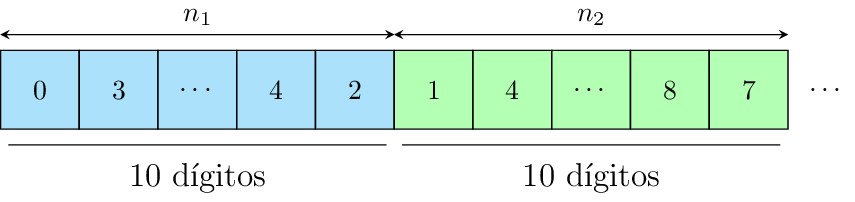
\includegraphics[width=0.8\linewidth]{Tesis UNAM/graficas/PCC/PCC.png}
        \centering
        \caption{Diagrama general de suceciones  de tamaño $n_i$ con 10 dígitos cada una.}
        \label{fig:PCC}
    \end{figure}





\subsection*{Prueba de brechas}

Una forma intuitiva de detectar dependencias sutiles o sesgos de
uniformidad en una secuencia de números pseudoaleatorios
$\{U_i\}_{i\ge 1}\subset(0,1)$ consiste en estudiar
\emph{cuántos intentos se necesitan para volver a obtener un “éxito”, para un experimento determinado}.  
La \textbf{prueba de brechas} (\textit{gaps test}) formaliza esta idea:

\begin{itemize}
    \item Se fija de antemano un sub-intervalo arbitrario $(\alpha,\beta)\subset(0,1)$,
        con $$0<\alpha<\beta<1,$$ y se declara \emph{éxito} cada vez que
        $U_i\in(\alpha,\beta)$.
    \item Entre dos éxitos consecutivos se cuentan los \emph{fracasos}
        (los $U_i$ que caen fuera de $(\alpha,\beta)$).  
        A dicha cantidad le asociamos una variable aleatoria y la denotamos por $B_n$.
        
    \item Se recorre la sucesión $U_{1},U_{2},\dots$ y agrupan las observaciones en bloques.
    
    \item El primer bloque termina con el primer $U_i\in(\alpha,\beta)$.
          \item El número de fracasos \emph{previos} a ese éxito se registra como
                \[
                    B_{1} \;=\;
                    |\{\,U_1,\dots,U_{i-1}\notin(\alpha,\beta)\}|.
                \]
    \item Tras cada éxito se reinicia el conteo, obteniéndose así la muestra
                $B_1,B_2,B_3,\dots$
    \end{itemize}
    
En la \Cref{fig:brech} tenemos un ejemplo sencillo con los primeros 8 términos de la sucesión de números generados. En este caso $U_{4}$ es el primer valor dentro de $(\alpha,\beta)$, por lo que $B_{1}=3$; el siguiente éxito es $U_{5}$ y la distancia en intentos entre $U_{4}$ y $U_{5}$ genera $B_{2}$, y así sucesivamente. \\

\begin{figure}[h!]                   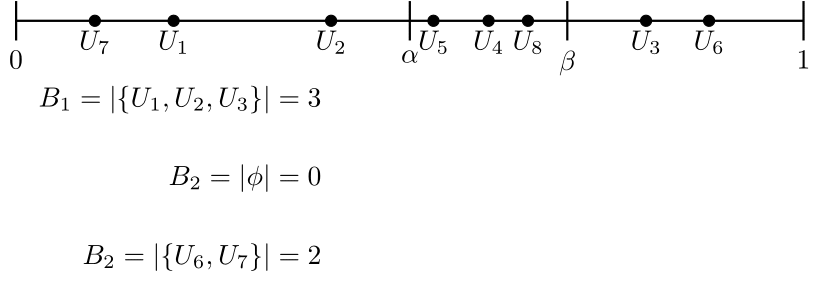
\includegraphics[width=0.8\linewidth]{Tesis UNAM/graficas/PG/PG.png}
        \centering
         \caption{Diagrama de Brechas en una sucesion $\{U_i\}_{1\leq i\leq 8}$.}
         \label{fig:brech}
    \end{figure}


Si los $U_i$ son realmente independientes y uniformes,
la probabilidad de éxito es constante $p=\beta-\alpha=\mathbb{P}\bigl(U_i \in (\alpha,\beta)\bigr)$
y cada $B_j$ debería seguir una distribución geométrica
      \[
            B_j \sim \operatorname{Geom}(p),
            \qquad
            \mathbb{P}(B_j = \ell) \;=\; (1-p)^{\ell}\,p,
            \quad \ell = 0,1,2,\dots
        \]
Además, la independencia implica que los $B_j$ son entre sí independientes.
La prueba compara la distribución empírica de las $B_j$'s con la distribución geométrica. 

\subsection{Distribuciones invariantes}
%% Todos los parametros racionales son ciclos 
En esta sección analizaremos el comportamiento del mapeo aplicado a variables aleatorias, es decir, el espacio de estados $E$ es ahora el conjunto de las variables aleatorias con soporte en $[0,1]$. El primer resultado que probaremos es el siguiente. 
\begin{proposition}\label{prop:log_unif}
Si $X$ es una variable aleatoria con distribución $Beta\left(\frac{1}{2},\frac{1}{2}\right)$, entonces es invariante al mapeo logístico, es decir, la variable aleatoria $Y$ definida como  $$Y:=\phi(X)$$ con $\phi$ la función descrita por el mapeo logístico \ref{eq:log} también tiene distribución $Beta\left(\frac{1}{2},\frac{1}{2}\right)$.
\end{proposition}
% \begin{remark}
%     Diremos que la variable aleatoria $X$ tiene distribución
% $\mathrm{Beta}(\alpha,\beta)$, con parámetros $\alpha>0$ y $\beta>0$, si su función
% de densidad es
% $$
% f_X(x;\alpha,\beta)=
% \begin{cases}
% \dfrac{x^{\alpha-1}(1-x)^{\beta-1}}{B(\alpha,\beta)}, & 0<x<1,\\[6pt]
% 0, & \text{en otro caso},
% \end{cases}
% $$
% donde $B(\alpha,\beta)$ es la función beta,
% $$
% B(\alpha,\beta)=\int_{0}^{1} t^{\alpha-1}(1-t)^{\beta-1}\,dt
% =\dfrac{\Gamma(\alpha)\,\Gamma(\beta)}{\Gamma(\alpha+\beta)}.
% $$
% \end{remark}
\begin{proof}
Observemos que la función de distribución acumulada de $Y$ está dada por \begin{align*}
    F_Y(y)=P(Y\leq y)=P(\phi(X)\leq y)
\end{align*}
los valores de $X$ que hacen posible la desigualdad dentro de la probabilidad son aquellos que están antes de la primera intersección del mapeo con la horizontal $y$ y los que están después de la segunda intersección, pues el mapeo es creciente para $X\leq \frac{1}{2}$ y decreciente para $X>\frac{1}{2}$, véase la Figura \ref{fig:log_proof}. Así, calculando dichas intersecciones obtenemos que los valores son $X_1=\frac{1-\sqrt{1-y}}{2}$ y $X_2=\frac{1+\sqrt{1-y}}{2}$, quedando así 
\begin{align*}
    F_Y(y)=&F_X\left(\frac{1-\sqrt{1-y}}{2}\right)+\left[1-F_X\left(\frac{1+\sqrt{1-y}}{2}\right)\right]
\end{align*}

\begin{figure}[h]
    \centering
    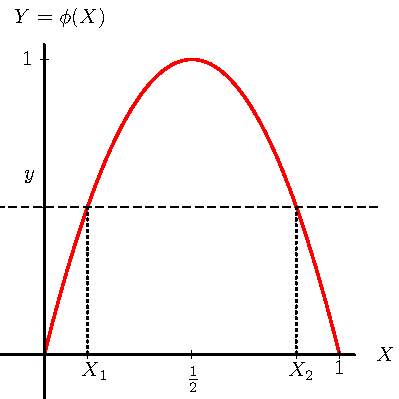
\includegraphics[width=0.40\textwidth]{Tesis UNAM/graficas/Logist/log_proof.pdf}
    \caption{Gráfica del mapeo de logisitico. Un número $y$ en $[0,1]$ tiene dos preimágenes, $X_1=\frac{1-\sqrt{1-y}}{2}$ y $X_2=\frac{1+\sqrt{1-y}}{2}$. Por lo tanto, los intervalos que tienen imágenes menores o iguales a $y$ son $\left[0,\frac{1-\sqrt{1-y}}{2}\right]$ y $\left[\frac{1+\sqrt{1-y}}{2},1\right]$.}
    \label{fig:log_proof}
\end{figure} 


Calculando la función de densidad de $Y$, derivando $F_Y$ y recordando que $X$ está distribuida $Beta\left(\frac{1}{2},\frac{1}{2}\right)$, obtenemos
\begin{align*}
f_Y(y) &= \frac{d}{dy} F_Y(y) \\
       &= \frac{d}{dy} \left[ F_X\left( \frac{1 - \sqrt{1 - y}}{2} \right) + 1 - F_X\left( \frac{1 + \sqrt{1 - y}}{2} \right) \right] \\
       &= \frac{1}{4} (1 - y)^{-1/2} \left[ f_X\left( \frac{1 - \sqrt{1 - y}}{2} \right) + f_X\left( \frac{1 + \sqrt{1 - y}}{2} \right) \right] \\
       &= \frac{(1 - y)^{-1/2}}{4B\left( \frac{1}{2}, \frac{1}{2} \right)} \left[ \left( \frac{1 - \sqrt{1 - y}}{2} \right)^{-1/2}\left( \frac{1 + \sqrt{1 - y}}{2} \right)^{-1/2} \right. \\
       & \qquad\qquad\qquad\quad \left. + \left( \frac{1 + \sqrt{1 - y}}{2} \right)^{-1/2}\left( \frac{1 - \sqrt{1 - y}}{2} \right)^{-1/2} \right] \\
       &= \frac{(1 - y)^{-1/2}}{2B\left( \frac{1}{2}, \frac{1}{2} \right)} \left[ \left( 1 - (1 - y) \right)^{-1/2} + \left( 1 - (1 - y) \right)^{-1/2} \right] \\
       &= \frac{(1 - y)^{-1/2}}{2B\left( \frac{1}{2}, \frac{1}{2} \right)} \left[ 2y^{-1/2} \right]=  \frac{1}{B\left( \frac{1}{2}, \frac{1}{2} \right)}  y^{-1/2}(1 - y)^{-1/2} \\
\end{align*}
 Por tanto, $Y$ también tiene distribución $Beta\left(\frac{1}{2},\frac{1}{2}\right)$. 
\end{proof}
Probar que la densidad $Beta\left(\frac{1}{2},\frac{1}{2}\right)$ no solo es un punto fijo para el sistema, sino que es un punto fijo estable queda fuera de los límites de este texto. Sin embargo, en el capítulo de resultados hay una sección dedicada a este cuestionamiento.  



\subsubsection{Mapeo tienda}
El mapeo tienda se define con la tupla $(\mathbb{N},[0,\frac{\mu}{2}],\phi)$, siendo su función de evolución:
\begin{equation}
    \label{eq:tent}
\phi(x_{n}) = 
\begin{cases} 
\mu x_n & \text{si } 0 \le x_n \le \frac{1}{2} \\
\mu (1 - x_n) & \text{si } \frac{1}{2} < x_n \le 1 
\end{cases}
\end{equation}
donde $\mu$ es un parámetro que determina el comportamiento del sistema. Debido a que se busca generar números aleatorios en el intervalo $[0,1]$, la elección del parámetro es $\mu=2$.
\begin{figure}[h]
    \centering
    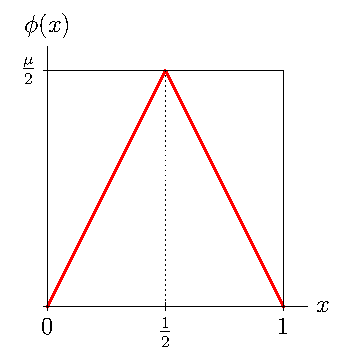
\includegraphics[width=0.40\textwidth]{Tesis UNAM/graficas/Tent/tent.pdf}
    \caption{Gráfica del mapeo tienda \ref{eq:tent}. Recibe su nombre gracias a que su gráfica parece una tienda de campaña.}
    \label{fig:tent_proof}
\end{figure} 

Algunas características de este mapeo son:

\begin{itemize}
    \item Si $\mu<1$ entonces el origen es el único unto fijo y es atractor.
    \item Si $\mu=1$, se cumple que si $x<\frac{1}{2}$, entonces $x$ es punto fijo.
    % La sucesión de bifrcaciones en estos sistemas es la misma salvo por una constante.
    \item Si $1<\mu<2$, existen dos puntos fijos en el sistema: $x^*_1=0$ y $x^*_2=\frac{\mu}{\mu +1}$ y ambos son puntos fijos inestables.
    \item Si $\mu=2$, la función de evolución del mapeo tienda \ref{eq:tent} es caótica\footnote{La prueba puede consultarse en \cite{KingMendez2014}.} en el intervalo [0,1], segun la definición \ref{def:caos}.
\end{itemize}


Este mapeo al igual que el logístico \ref{eq:log} es conocido por su capacidad para generar secuencias que muestran propiedades de aleatoriedad \cite{Schuster2005}. Variaciones de este mapeo han sido una herramienta muy utilizada en la generación de números pseudoaleatorios \cite{Callegari1997}.



\begin{figure}[h!]
    \centering
    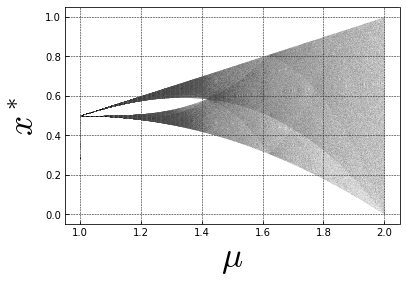
\includegraphics[width=12cm]{Tesis UNAM/graficas/Tent/tent_bif.png}
    \caption{Bifrcaciones del mapeo tienda.}
    \label{fig:bif-log}
\end{figure} 



\subsubsection{Distribuciones invariantes al mapeo tienda}
%% Todos los parametros racionales son ciclos 
En esta sección se hace un análisis similar al del comportamiento del mapeo logístico con una densidad $Beta(\frac{1}{2},\frac{1}{2})$. La densidad uniforme es el punto fijo en este sistema.
\begin{proposition}\label{prop:tent_unif}
Si $X$ es una variable aleatoria con distribución uniforme en el intervalo $[0,1]$, entonces es invariante al mapeo tienda, es decir, la variable aleatoria $Y$ definida como  $$Y:=\phi(X)$$ con $\phi$ la función descrita por \ref{eq:tent} también tiene distribución uniforme en $[0,1]$.
\end{proposition}
\begin{proof}
Observemos que la función de distribución acumulada de $Y$ está dada por \begin{align*}
    F_Y(y)=P(Y\leq y)=P(\phi(X)\leq y)
\end{align*}
los valores de $X$ que hacen posible la desigualdad dentro de la probabilidad son aquellos que están antes de la primera intersección del mapeo con la horizontal $y$ y los que están después de la segunda intersección, pues el mapeo es creciente para $X\leq \frac{1}{2}$ y decreciente para $X>\frac{1}{2}$, véase la Figura \ref{fig:tent_proof}. Así, calculando dicha intersección obtenemos que los valores son $X_1=\frac{y}{2}$ y $X_2=1-\frac{y}{2}$, quedando así 
\begin{align*}
    F_Y(y)=&F_X\left(\frac{y}{2}\right)+\left[1-F_X\left(1-\frac{y}{2}\right)\right]
\end{align*}

\begin{figure}[h]
    \centering
    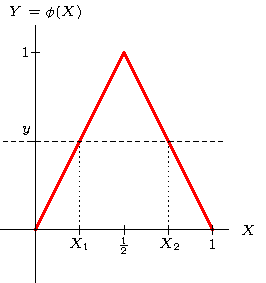
\includegraphics[width=0.40\textwidth]{Tesis UNAM/graficas/Tent/tent_proof.pdf}
    \caption{Gráfica del mapeo de "tienda de campaña". Un número $y$ en $[0,1]$ tiene dos preimágenes, $X_1=\frac{y}{2}$ y $X_2=1-\frac{y}{2}$. Por lo tanto, los intervalos que tienen imágenes menores o iguales a $y$ son $[0,\frac{y}{2}]$ y $[1-\frac{y}{2},1]$.}
    \label{fig:tent_proof}
\end{figure} 

Calculando la función de densidad de $Y$, derivando $F_Y$ obtenemos 
\begin{equation}
    f_Y(y)=\frac{1}{2}\left[f_X\left(\frac{y}{2}\right)+f_X\left(1-\frac{y}{2}\right)\right]
    \label{eq:dens_Y_tent}
\end{equation}
Observemos que la densidad uniforme se define como:
\[f_X(y)=\mathbf{1}_{[0,1]}(y)\] siendo \(\mathbf{1}_{[0,1]}(y)\) la función indicadora que se define como:
\[
\mathbf{1}_{[0,1]}(y) = 
\begin{cases}
1 & \text{si } 0 \leq y \leq 1, \\
0 & \text{en otro caso}.
\end{cases}
\]
Entonces \[f_X\left(\frac{y}{2}\right)=\mathbf{1}_{[0,1]}\left(\frac{y}{2}\right)=
\begin{cases}
1 & \text{si } 0 \leq y/2 \leq 1, \\
0 & \text{en otro caso}.
\end{cases}\]


Simplificando la desigualdad \(0 \leq y/2 \leq 1\) como \(
0 \leq y \leq 2,
\)
tenemos que:
\[
f_X\left(\frac{y}{2}\right)=\mathbf{1}_{[0,1]}\left(\frac{y}{2}\right) = 
\begin{cases}
1 & \text{si } 0 \leq y \leq 2, \\
0 & \text{en otro caso}.
\end{cases}
\]

Esto muestra que $f_X\left(\frac{y}{2}\right)$ es en realidad la función indicadora del intervalo \([0,2]\), es decir:
\[
f_X\left(\frac{y}{2}\right) = \mathbf{1}_{[0,2]}(y).
\]

sin embargo $X$ tiene soporte en $[0,1]$ y el dominio y contradominio de $\phi$ es el mismo intervalo. Algo análogo sucede con $f_X\left(1-\frac{y}{2}\right)$. Finalmente, vemos que la expresión de la densidad de $Y$ (\ref{eq:dens_Y_tent}) es la constante uno y por tanto, $Y$ también tiene distribución uniforme. 
\end{proof}


  
\end{document}
